\documentclass[]{elsarticle} %review=doublespace preprint=single 5p=2 column
%%% Begin My package additions %%%%%%%%%%%%%%%%%%%
\usepackage[hyphens]{url}



\usepackage{lineno} % add
\providecommand{\tightlist}{%
  \setlength{\itemsep}{0pt}\setlength{\parskip}{0pt}}

\bibliographystyle{elsarticle-harv}
\biboptions{sort&compress} % For natbib
\usepackage{graphicx}
\usepackage{booktabs} % book-quality tables
%%%%%%%%%%%%%%%% end my additions to header

\usepackage[T1]{fontenc}
\usepackage{lmodern}
\usepackage{amssymb,amsmath}
\usepackage{ifxetex,ifluatex}
\usepackage{fixltx2e} % provides \textsubscript
% use upquote if available, for straight quotes in verbatim environments
\IfFileExists{upquote.sty}{\usepackage{upquote}}{}
\ifnum 0\ifxetex 1\fi\ifluatex 1\fi=0 % if pdftex
  \usepackage[utf8]{inputenc}
\else % if luatex or xelatex
  \usepackage{fontspec}
  \ifxetex
    \usepackage{xltxtra,xunicode}
  \fi
  \defaultfontfeatures{Mapping=tex-text,Scale=MatchLowercase}
  \newcommand{\euro}{€}
\fi
% use microtype if available
\IfFileExists{microtype.sty}{\usepackage{microtype}}{}
\usepackage{graphicx}
% We will generate all images so they have a width \maxwidth. This means
% that they will get their normal width if they fit onto the page, but
% are scaled down if they would overflow the margins.
\makeatletter
\def\maxwidth{\ifdim\Gin@nat@width>\linewidth\linewidth
\else\Gin@nat@width\fi}
\makeatother
\let\Oldincludegraphics\includegraphics
\renewcommand{\includegraphics}[1]{\Oldincludegraphics[width=\maxwidth]{#1}}
\ifxetex
  \usepackage[setpagesize=false, % page size defined by xetex
              unicode=false, % unicode breaks when used with xetex
              xetex]{hyperref}
\else
  \usepackage[unicode=true]{hyperref}
\fi
\hypersetup{breaklinks=true,
            bookmarks=true,
            pdfauthor={},
            pdftitle={Inducing Non-Orthogonal and Non-Linear Decision Boundaries in Decision Trees via Interactive Basis Functions},
            colorlinks=true,
            urlcolor=blue,
            linkcolor=magenta,
            pdfborder={0 0 0}}
\urlstyle{same}  % don't use monospace font for urls

\setcounter{secnumdepth}{0}
% Pandoc toggle for numbering sections (defaults to be off)
\setcounter{secnumdepth}{0}
% Pandoc header
\usepackage{float}
\usepackage[nomarkers,figuresonly]{endfloat}
\floatplacement{figure}{H}
\usepackage{booktabs}



\begin{document}
\begin{frontmatter}

  \title{Inducing Non-Orthogonal and Non-Linear Decision Boundaries in Decision
Trees via Interactive Basis Functions}
    \author[McMaster University]{Antonio Paez\corref{c1}}
   \ead{paezha@mcmaster.ca} 
   \cortext[c1]{Corresponding Author}
    \author[Universidad Politecnica de Cartagena]{Fernando Lopez}
   \ead{fernando.lopez@upct.es} 
  
    \author[Universidad Politecnica de Cartagena]{Manuel Ruiz}
   \ead{manuel.ruiz@upct.es} 
  
    \author[Universidad de Murcia]{Maximo Camacho}
   \ead{m.camacho@um.es} 
  
      \address[McMaster University]{School of Geography and Earth Sciences, 1280 Main Street West, Hamilton
ON, Canada L8S 4K1}
    \address[Universidad Politecnica de Cartagena]{Facultad de Ciencias de la Empresa, Dept. de Métodos Cuantitativos e
Informáticos, Calle Real, 3, 30201 Cartagena, Murcia, España}
    \address[Universidad de Murcia]{Facultad de Economía y Empresa, Dept. de Métodos Cuantitativos para la
Economía y la Empresa, 30100 Murcia, Murcia, España}
  
  \begin{abstract}
  Decision Trees (DTs) are a machine learning technique widely used for
  regression and classification purposes. Conventionally, the decision
  boundaries of Decision Trees are orthogonal to the features under
  consideration. A well-known limitation of this is that the algorithm may
  fail to find optimal partitions, or in some cases any partitions at all,
  depending on the underlying distribution of the data. To remedy this
  limitation, several modifications have been proposed that allow for
  oblique decision boundaries. The objective of this paper is to propose a
  new strategy for generating flexible decision boundaries by means of
  interactive basis functions (IBFs). We show how oblique decision
  boundaries can be obtained as a particular case of IBFs, and in addition
  how non-linear decision boundaries can be induced. One attractive aspect
  of the strategy proposed in this paper is that training Decision Trees
  with IBFs does not require custom software, since the functions can be
  precalculated for use in any existing implementation of the algorithm.
  Since the underlying mechanisms remain unchanged there is no substantial
  computational overhead compared to conventional trees. Furthermore, this
  also means that IBFs can be used in any extensions of the Decision Tree
  algorithm, such as evolutionary trees, boosting, and bagging. We conduct
  a benchmarking exercise to show how the use of IBFs can often improve
  the performance of models. In addition, we present three empirical
  applications that illustrate the approach in classification and
  regression. As part of discussing the empirical applications, we
  introduce a device called \emph{decision charts} to facilitate the
  interpretation of DTs with IBFs. Finally, we conclude the paper by
  outlining some directions for future research.
  \end{abstract}
  
 \end{frontmatter}

\section{1 Introduction}\label{introduction}

Decision Trees (DTs) are a popular machine learning technique used both
for regression and classification purposes (Loh 2011; James et al.
2013). A DT is trained by means of a training dataset that provides a
set of independent variables (or \emph{features}) used to create
recursive partitions of the decision space. This is achieved by locally
optimizing at each step a loss function that depends on the type of
problem (i.e., regression or classification) and/or the specific
implementation of the algorithm (i.e., an entropy function for C4.5 and
a gini index for CART; see Loh 2011).

Decision Trees find applications in a variety of domains, including,
inter alia, transportation (e.g., Ghasri, Rashidi, and Waller 2017),
physical geography (e.g., Praskievicz 2018), engineering (e.g., Bektas,
Carriquiry, and Smadi 2013; Suhail, Denton, and Zwiggelaar 2018), and
environmental sciences (e.g., Choubin et al. 2018). There are several
characteristics that make DTs an appealing modeling approach. Notably,
DTs are more intuitive than linear/logistic regression (James et al.
2013, 315) and have much greater interpretability than, for instance,
artificial neural networks and support vector machines (Yang et al.
2017, 354). In addition, in some settings DTs provide a reasonable
heuristic for human decision making (James et al. 2013, 315). Finally,
although no single technique can be expected to be uniformly superior in
every case, the performance of DTs has been shown to be competitive
with, and in some cases superior to, alternatives such as linear
regression, logistic regression, support vector machines, and artificial
neural networks (e.g., Kurt, Ture, and Kurum 2008; Choubin et al. 2018;
Yang et al. 2017).

One characteristic of DTs as conventionally implemented, is that
partitions of the variable space are usually done orthogonally to the
features. In this way, the partitions are a set of rectangular
\(p\)-dimensional prisms,or hyperboxes. While this is done to reduce the
search space of the algorithm, it has the downside that it may fail to
find appropriate partitions, and in some extreme cases, to find any
partitions at all. In this case, the performance of the algorithm tends
to be mediocre. Accordingly, a number of proposals have aimed at
ameliorating this situation by inducing oblique partitions (e.g.,
Murthy, Kasif, and Salzberg 1994; Wickramarachchi et al. 2016; Cantu-Paz
and Kamath 2003).

The objective of this paper is to introduce a novel strategy for
non-orthogonal partition of variable space in the training of DTs. The
approach is based on the use of interactive basis functions (IBFs). We
will show that oblique partitions result as a particular case of an IBF.
Moreover, depending on the basis function selected, non-linear
partitions are also possible. The modeling strategy proposed in this
paper is attractive because the basis functions can be precalculated and
then used as an input to any decision tree algorithm. Since only the
inputs to the algorithm change, this implies that 1) the underlying
algorithm is not changed and therefore any existing DT software can be
used; and 2) basis functions can be used in many existing
implementations of DTs, including evolutionary trees, bagging, and
boosting.

The structure of the paper is as follows. In the {[}background
section{]}{[}Background{]} we first review some technical aspects of
decision trees and motivate the problem. This is followed by a
discussion of {[}basis functions{]}{[}Interactive Basis Functions{]} and
how they can be employed to induce oblique linear and non-linear
partitions. Next, we discuss some {[}practical aspects{]}{[}Practical
Considerations{]} of implementing IBFs before conducting a
{[}benchmarking experiment{]}{[}Benchmarking{]} the assess the
performance or DTs with IBFs by means of a set of publicly available
empirical datasets. The results indicate that inducing oblique and/or
non-linear partitions using basis functions can improve the performance
of the technique and/or produce more parsimonious models. We then
illustrating the {[}application{]}{[}Sample Applications{]} of IBFs by
means of three empirical examples. Finally, we
{[}conclude{]}{[}Conclusions and Directions for Future Research{]} the
paper by summarizing our findings and suggesting some directions for
future research.

Given the simplicity and ease of implementation of the modeling
strategy, the development presented in this paper should be of interest
for users of DTs who wish to improve the performance of their models at
a relatively modest computational cost.

\section{2 Background}\label{background}

We begin in this section by formally describing the DT algorithm. This
will serve to motivate subsequent sections of the paper.

A decision tree is a regression/classification algorithm which models a
response variable \(Y\) (which could be quantitative or qualitative)
from a vector of \(p\) features, \(X=(X_{1},\dots,X_{p})\), where
\(X\in \mathrm{R}^{p}\). The algorithm operates by recursively
partitioning the space of the features into a set of \(M\) regions
\(R_{m}\), \(m=1,...,M\).

To state the basic notation, let us start by considering a binary tree
model with \(M\) terminal nodes, each of which
\(m\in \left\{ 1,...,M \right\}\) represents a branch of the tree that
is characterized by \(m^{\ast}\) internal splits. The parameter space
that characterizes each branch is
\(\theta_{m}^{m^{\ast }}=\left(v_{m,1}^{d_{1}},s_{m,1},...,v_{{m,m}^{\ast }}^{d_{m^{\ast }}},s_{{m,m}^{\ast}} \right)\),
where \(X_{v_{m,i}}\) is the splitting variable at the internal split
\(i\) of the terminal node \(m\), with
\(v_{mi}\in \left\{ 1,...,P \right\}\), \(d_{i}=0\) if
\(X_{v_{m,i}}<s_{m,i}\) and \(d_{i}=1\) if \(X_{v_{m,i}}>s_{m,i}\),
\(s_{m,i}\) is the splitting point, and
\(i\in \left\{ 1,...,m^{\ast } \right\}\). The parameter space of trees
with \(M\) terminal nodes, \(\Theta_{M}\), is formed by the collection
of all the combinations of
\(\theta_{m}=\bigcup\limits_{j=1}^{m^{\ast }}\theta_{m}^{j}\),
\(\Theta_{M}=\bigcup\limits_{m=1}^M \theta_{m}\). In this way, a tree is
a collection of branches, each of which ends up in a terminal node, that
characterizes the partitions or regions through \(\theta_{m}\).

The objective of the recursive partitioning mechanism is to try to find
optimal partitions in the search space of the features as follows. The
path of the partitions determined by each branch is:

\[
\theta_{m}^{j}=\theta_{m}^{j-1}\bigcup \left( v_{m,j}^{d_{j}},s_{m,j} \right) ,
\]

Within this framework, each branch \(m\) is a collection of sequential
partitions \(\theta_{m}^{j}\), \(j=1,\dots,m^{\ast }\). For each of
these partitions, we define a prediction function
\(f\left( X,\theta _{m}^{j} \right)\), which typically is a central
tendency measure of the values of the dependent variable conditional to
that region. The goal is to find a decision tree that optimizes some
tradeoff between prediction performance, measured by a loss function,
\(loss\left\{ Y,f\left( X,\theta_{m}^{j} \right) \right\}\), and a
measure of the complexity of the tree,
\(comp\left( \theta_{m}^{j} \right)\),
\(\hat{\theta}_{m}^{j}=\arg \left[ loss\left\{ Y,f\left( X,\theta_{m}^{j} \right)\right\}+comp\left( \theta_{m}^{j} \right) \right].\)

In practice, the recursion ends when any additional partitions result in
subsamples below a minimum number of cases (e.g., less than five cases).
Operating in this way, the recursive partitioning method produces
partitions that are orthogonal to the \(p\) features, and thus results
in a total of \(M\) \(p\)-dimensional rectangular prisms, or hyperboxes
(see Figure 1 \ref{fig:fig1-example} for a prototypical decision tree
with two features \(X_1\) and \(X_2\)).

\begin{figure}[htbp]
\centering
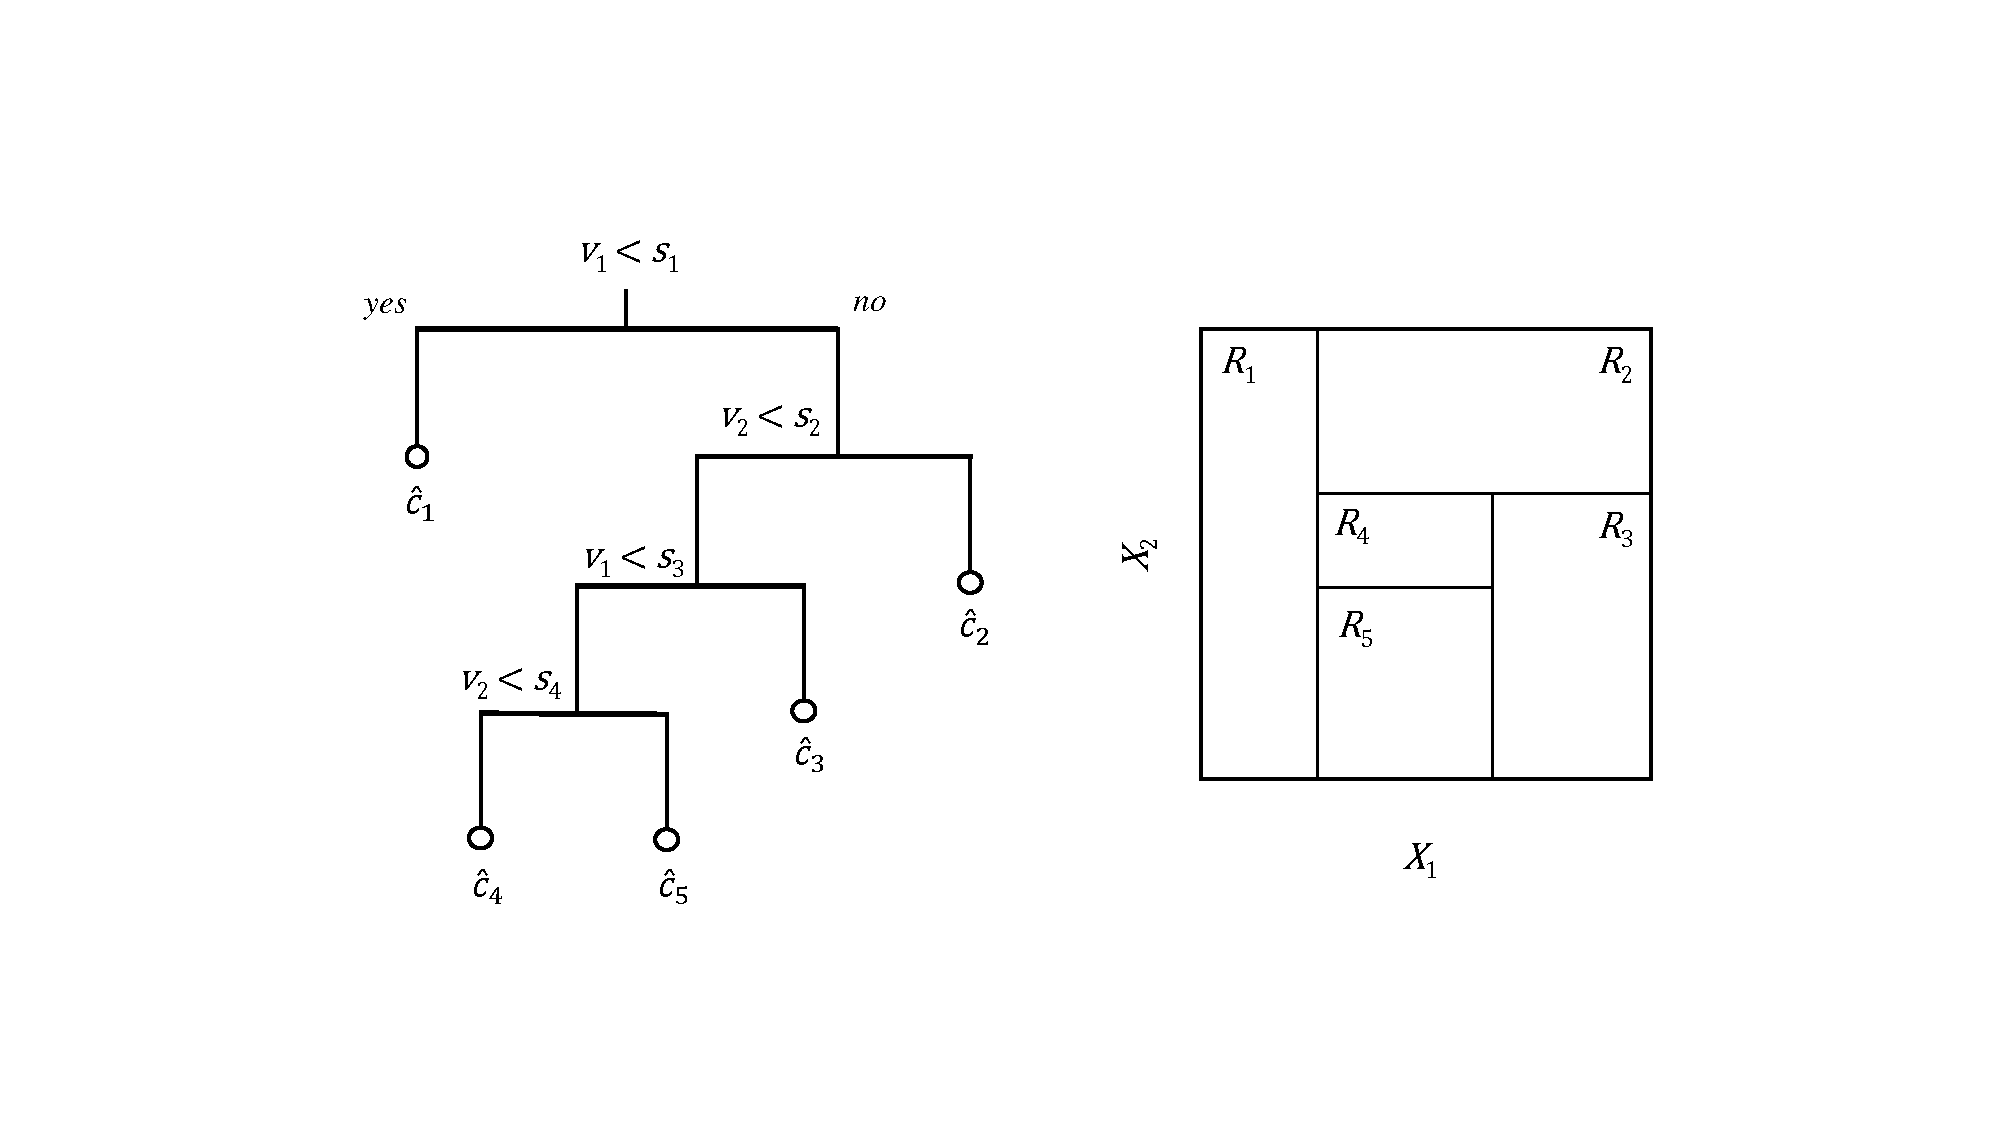
\includegraphics{fig1-example.pdf}
\caption{\label{fig:fig1-example}Prototypical Decision Tree}
\end{figure}

Despite its advantages, it is not difficult to find examples where
orthogonal recursive partitioning does not work. Consider the situation
depicted in Figure \ref{fig:fig2-chessboard}, a simple classification
problem with \(p=2\) features. It is straightforward to see that in this
case the algorithm fails to find an initial partition, as the loss
function on the resulting subsets cannot be reduced by any first split.
This situation, on the other hand, is easily avoided if oblique splits
are used. In this case an optimal split can be found at the first step,
as illustrated by the candidate split shown with a dashed line in the
figure.

\begin{figure}[htbp]
\centering
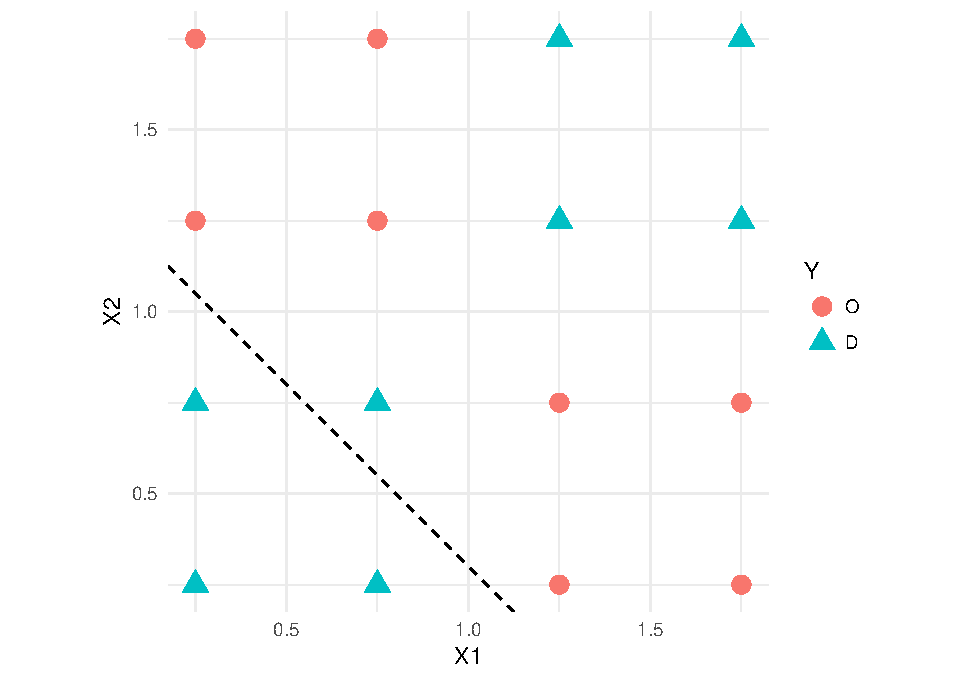
\includegraphics{Trees_with_Base_Functions_files/figure-latex/fig2-chessboard-1.pdf}
\caption{\label{fig:fig2-chessboard}Chessboard example}
\end{figure}

Motivated by the challenge posed by situations such as the one in Figure
\ref{fig:fig2-chessboard}, and more generally to better capture
non-orthogonal decision boundaries, previous research has seen the
development of numerous methods to induce oblique decision boundaries
for trees (see Cantu-Paz and Kamath 2003; and Wickramarachchi et al.
2016 for an overview).

As discussed by Wickramarachchi et al. (2016), some algorithms used to
induce oblique partitions identify candidate partition boundaries based
on the statistical properties of the data. For instance, a number of
algorithms use the orientation of the classes as given by their first
principal component (Henrichon and King-Sun 1969), the Household
projection matrix (Wickramarachchi et al. 2016), or Fisher's linear
discriminant (Friedman, Bentley, and Finkel 1977). New features are
added to the problem, and the conventional orthogonal partition
mechanism is retained. Other algorithms are based on optimization
approaches, which could be deterministic or stochastic. CART-LC (Breiman
et al. 1984) is an example of the former, whereas Cantu-Paz and Kamath
(2003) with their use of genetic algorithms is an example of the latter.
The increase in complexity of these algorithms, and consequently their
computational burden, comes from the additional steps needed to conduct
additional statistical or optimization procedures. Finally, heuristic
approaches have also been used, for example by Manwani and Sastry (2012)
and Robertson, Price, and Reale (2013).

In the following section, we describe a novel strategy to induce oblique
(and possibly non-linear) decision boundaries via the application of
\emph{interactive basis functions} (IBFs). This modelling strategy adds
judiciously constructed features to the dataset while retaining the
conventional orthogonal partition mechanism.

\section{3 Interactive Basis Functions
(IBFs)}\label{interactive-basis-functions-ibfs}

Let us begin our discussion of basis functions by stating that the
search domain of a decision tree is contained by the features under
consideration. Put in other words, the features used for training
constitute the basis vectors for the problem. For instance, when the
number of features is \(p=2\), the search space is the plane formed by
the orthogonal axes of the features, and each feature is a basis vector.
Three features form a 3D basis, and so on. If we consider a feature as a
basis vector, a basis function is simply a transformation thereby. In
the simplest case, the basis function could be the identity: \[
b(X_1) = X_1
\] which is a particular case of a polynomial function, with \(a=1\): \[
b(X_1) = X_1^a
\]

Other basis functions can be defined as well, such as the exponential:
\[
b(X_1) = e^{X_1}
\]

Basis functions are commonly used in regression analysis, where they
have the effect of changing the properties of a regression plane. For
instance, a transformation from identity to the square of a variable has
the effect of changing the regression line to a parabola. Alas, the use
of basis functions in DTs does not have the same effect. To see why this
is so, consider the general case with \(K\) real functions
\(b_{i}:\mathbb{R}\rightarrow\mathbb{R}\) with \(i=1,\dots,K\) candidate
base functions. We will call \(\{b_1,b_2,\dots, b_K\}\) a set of basis
functions. Next proceed to enlarge the set of \(p\) features with \(T\)
new features obtained by means of basis functions:

\[
X^{\ast }=\left( X_{1},\dots,X_{p},X_{p+1},\dots ,X_{p+T} \right)
\]

where \(X^{\ast }\in \mathbb{R}^{p+T}\), and
\(X_{p+i}=b_{s_i}( X_{j_i})\), for \(i=1,\dots ,T\),
\(s_i\in \{1,\dots,K\}\) and \(j_i\in\{1,\dots,p\}\)

Notably, the standard recursive partitioning mechanism of Decision Trees
applied to any \(X_p\) in the augmented set \(T\) leads to partitions of
\(\left(p+T\right)\)-dimensional prisms. Furthermore, the projections of
these prisms in the subspace of \(\mathrm{R}^{p}\) defined by \(X\)
still reproduce a linear orthogothal partition of this space. Consider
an example with \(p=2\), that is \(X=\{X_1,X_2\}\). Moreover, \(T=1\)
and \(K=1\) with \(b_1(x)=x^2\), so that
\(X^\ast=\{X_1,X_2,X_3=X_1^2\}\). Whenever the partitioning mechanism
selects a split \(s\) in \(X_3\) (say, \(s=2\), the solid line in Figure
\ref{fig:fig3-simple-basis}), this split is projected in \(X\) as
\(X_1=\sqrt X_3\), which is a constant. As a consequence, any splits on
the dimension of the basis function is equivalent to finding an
orthogonal decision boundary on the original basis, in the present
example at \(\sqrt 2\) in \(X_1\) (dashed line).

\begin{figure}[htbp]
\centering
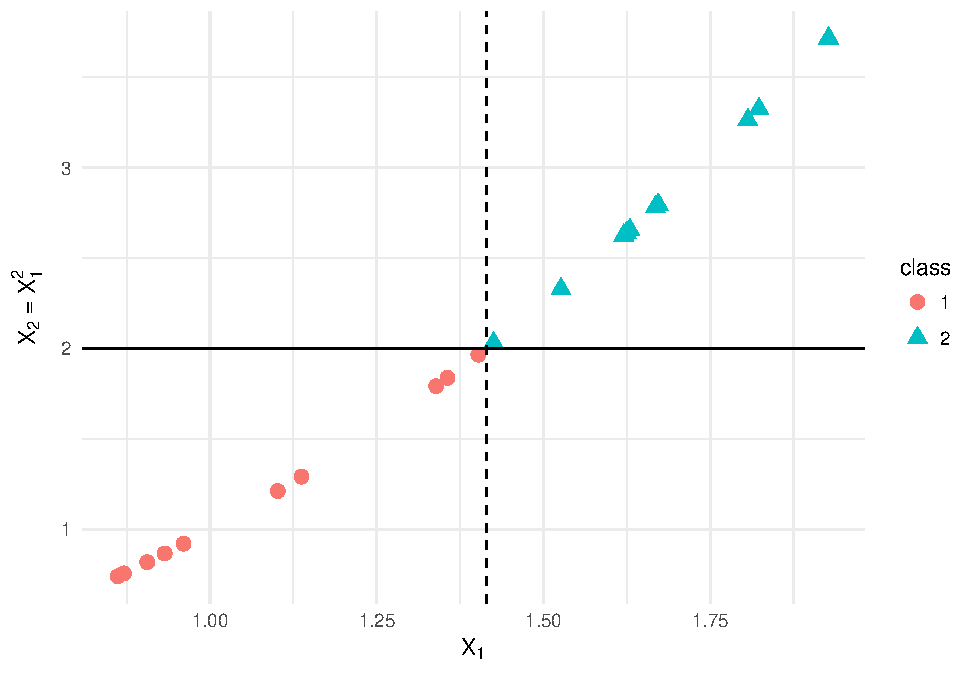
\includegraphics{Trees_with_Base_Functions_files/figure-latex/fig3-simple-basis-1.pdf}
\caption{\label{fig:fig3-simple-basis}Example of a basis function used
as a feature to train a Decision Tree}
\end{figure}

Since basis functions still produce orthogonal partitions in the
original basis, our proposal instead is to use interactive basis
functions in the construction of \(X^\ast\) for the tree under
consideration. These interactions can be identified by a set of \(D\)
functions that reproduce functional interactions of the transformations
of the features by the basis functions. Thus, these interaction
functions are defined as:

\[
\begin{array}{ccl}h_{i}:\mathbb{R}^{pK}&\longrightarrow&\mathbb{R}\\{\tiny (b_1(X_1),b_1(X_2)\dots, b_K(X_p))}&\leadsto &a\end{array}
\]

Under this setting define
\(X^{\ast }=\left( X_{1},\dots,X_{p},X_{p+1},\dots ,X_{p+D} \right)\),
with \(X_{p+i}=h_i(b_1(X_1),b_1(X_2)\dots, b_K(X_p))\), for
\(i=1,\dots ,D\). Therefore by applying the standard recursive
partitioning method to \(X^\ast\), its projection on \(X\) will provide
an oblique partition (also eventually non-linear as desired), which will
take into account the interactions among the features.

For example, in the case of \(p=2\), that is \(X=\{X_1,X_2\}\), \(T=1\),
\(K=1\) with \(b_1(x)=x\), \(D=1\) with
\(h_1(b_1(X_1),b_1(X_2))=b_1(X_1)+b_2(X_2)=X_1+X_2\) (i.e., an additivie
function) and \(X^{\ast }=\left( X_{1},X_{2},X_{3} \right)\) we obtain
that \(X_3=s\) is projected in the plane of the original basis as
\(X_2=s-X_1\), thus providing an oblique partition on that plane as
shown in Figure \ref{fig:fig4-additive-basis}.

\begin{figure}[htbp]
\centering
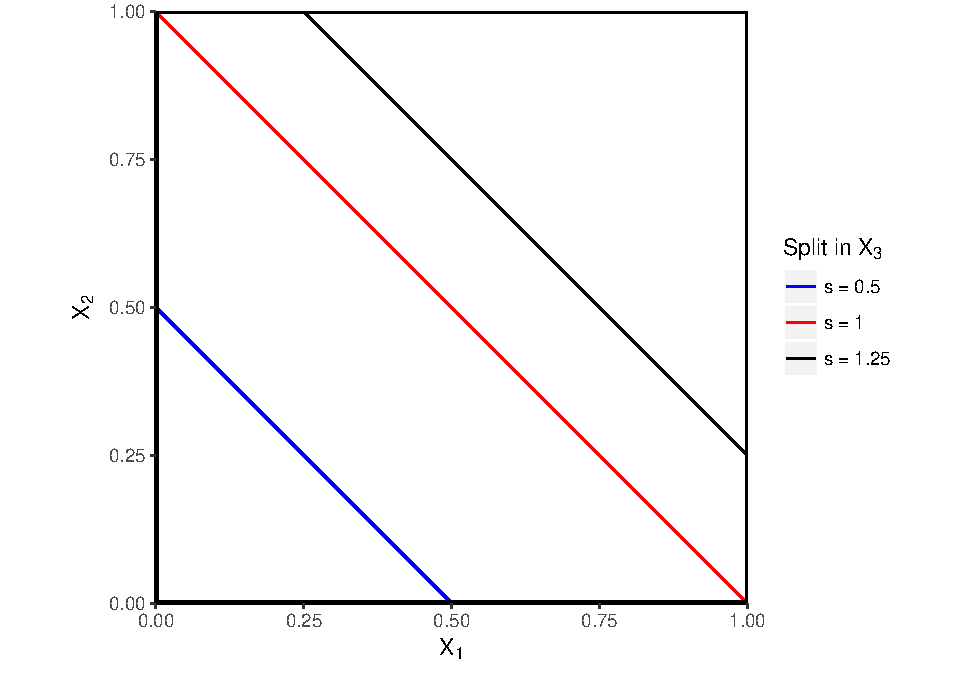
\includegraphics{Trees_with_Base_Functions_files/figure-latex/fig4-additive-basis-1.pdf}
\caption{\label{fig:fig4-additive-basis}Oblique basis function and
projections with different splitting points (s)}
\end{figure}

It is interesting to note that the framework provided by IBFs allows us
to induce, in addition to oblique partitions, non-linear decision
boundaries as well. This is done by projecting the equation
\(h_i(b_1(X_1),b_1(X_2)\dots, b_K(X_p))=a\) in the subspace
\(X=\{X_1, X_2,\dots, X_p\}\) generated by the features in the dataset.
For example, the IBF \(h_1(b_1(X_1),b_1(X_2))=b_1(X_1)b_2(X_2)\) with
\(b_1(x)=x\) leads to \(X_1X_2\). A split \(s\) in the dimension of this
multiplicative IBF fixes \(X_1X_2=s\), and therefore \(X_2=s/X_1\), thus
creating a hyperbolic partition, as shown in Figure
\ref{fig:fig5-hyperbolic-basis}.

\begin{figure}[htbp]
\centering
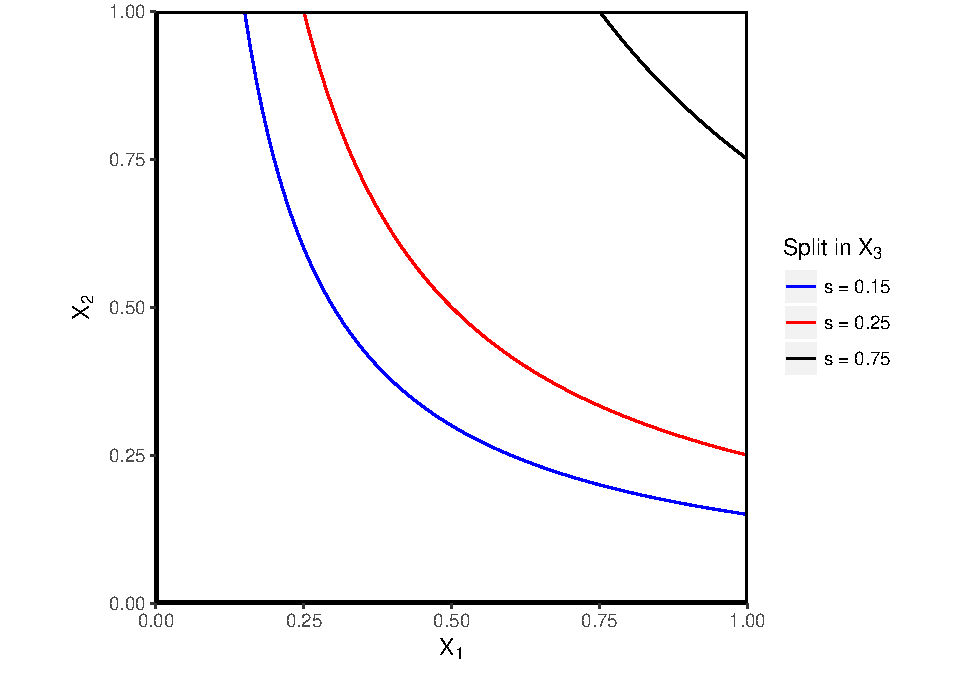
\includegraphics{Trees_with_Base_Functions_files/figure-latex/fig5-hyperbolic-basis-1.pdf}
\caption{\label{fig:fig5-hyperbolic-basis}Hyperbolic basis function and
projections with different splitting points (s)}
\end{figure}

As one final example (see Figure \ref{fig:fig6-radial-basis}), the IBF
\(h_1(b_1(X_1),b_1(X_2))=b_1(X_1)+b_2(X_2)\) with \(b_1(x)=x^2\) leads
to \(X_1^2 + X_2^2\). A split \(s\) in the dimension of the IBF fixes
\(X_1^2 + X_2^2=s\), and therefore \(X_2=\sqrt{s-X_1^2}\), thus creating
a radial partition.

\begin{figure}[htbp]
\centering
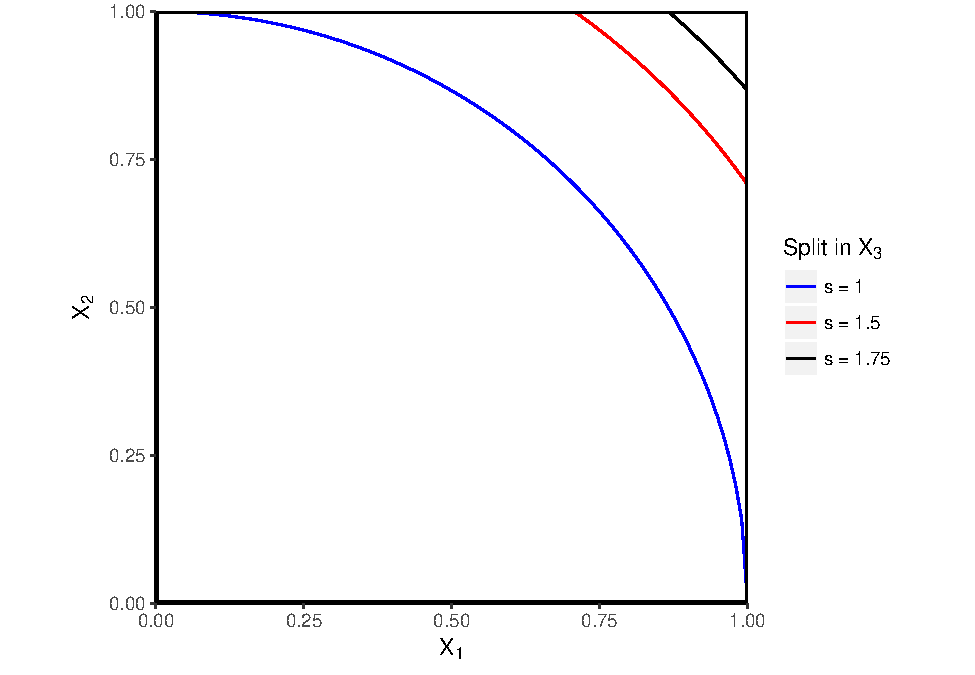
\includegraphics{Trees_with_Base_Functions_files/figure-latex/fig6-radial-basis-1.pdf}
\caption{\label{fig:fig6-radial-basis}Radial IBF and projections with
different splitting points (s)}
\end{figure}

It is worthwhile noting at this point that the additive function shown
in Figure \ref{fig:fig4-additive-basis} is similar to the case of linear
combinations used in the CART-LC algorithm (see Cantu-Paz and Kamath
2003), however without parameterizing the interactive basis function -
or, alternatively, implicitly assuming that \(a_1=a_2=1\): \[
h_1(b_1(X_1),b_1(X_2))=b_1(X_1)+b_2(X_2)=a_1X_1+a_2X_2
\]

In this way, the implementation of IBFs as non-parametric functions
leads to a semi-parametric version of DTs. With respect to the
complexity of the search, the introduction of IBFs increases the
complexity at each node of the tree (when using the conventional search
algorithm) by \(O(n(p+D))\), where \(n\) is the number of cases, \(p\)
is the number of features, and \(D\) is the number of IBFs under
consideration. Compare to the exaustive search for oblique decision
boundaries (\(O(2^p \times{n\choose{p}})\), in Murthy, Kasif, and
Salzberg 1994), or an algorithm such as HHCART, which has complexity of
\(O(Cp^2nlog(n))\) (where \(C\) is the number of classes in
classification problems, Wickramarachchi et al. 2016). As can be
appreciated, the increase in complexity with our approach is fairly
modest.

\section{4 Practical Considerations}\label{practical-considerations}

An important consideration in the practical implementation of IBFs
concerns the centering and/or scaling of the input features. Centering
and scaling are typically monotonical transformations of the data. For
instance, a feature vector can be centered on its minimum value or its
mean, thus shifting the origin. Scaling can be done for example by
scaling all values to the unit interval, or by dividing by the standard
deviation to normalize the scale.

Scaling and centering the features has no impact in the training of DT
with linear partitions, whether orthogonal or oblique. Any monotonic
transformation of the data will simply shift the splitting point that
creates a partition accordingly. The same does not necessarily happen
with non-linear partitions. Recall that the curvature \(\kappa\) of a
plane curve is related to the radius of the curve as follows for a given
arc length \(l\): \[
\kappa(l)=\frac{1}{R(l)}
\]

Intuitively, the curvature of a straight line is constant at zero. When
the radius of a curve for \(l\) is large the curvature is small, and
viceversa. It follows then that the geometric representation of a
non-linear partition in the subspace \(X\) depends on the origin (i.e.,
center) and scale in which the independent variables have been measured.
This effect is illustrated in Figure \ref{fig:fig7-curvature}, where a
set of radial IBFs are plotted. In one case (top panel) the features
\(X_1\) and \(X_2\) are measured in possibly different scales. Since the
origin for these variables is at zero, the radius of the curves is large
for partitions whithin the space of interest, and therefore the
partitions generated are locally quasi-linear. The bottom panel of the
figure shows analog radial IBFs, but now on features \(X'_1\) and
\(X'_2\). These features are obtained by centering variables \(X_1\) and
\(X_2\) on their minimum values, and scaling them to the unit length.
Now the radii of the IBFs are smaller, thus resulting on greater
curvature and locally non-linear partitions.

For this reason, we recommend centering and scaling all features prior
to analysis, in order to increase the chances that non-linear partitions
are effective, and reduce the possibility that they resemble linear
partitions locally.

\begin{figure}[htbp]
\centering
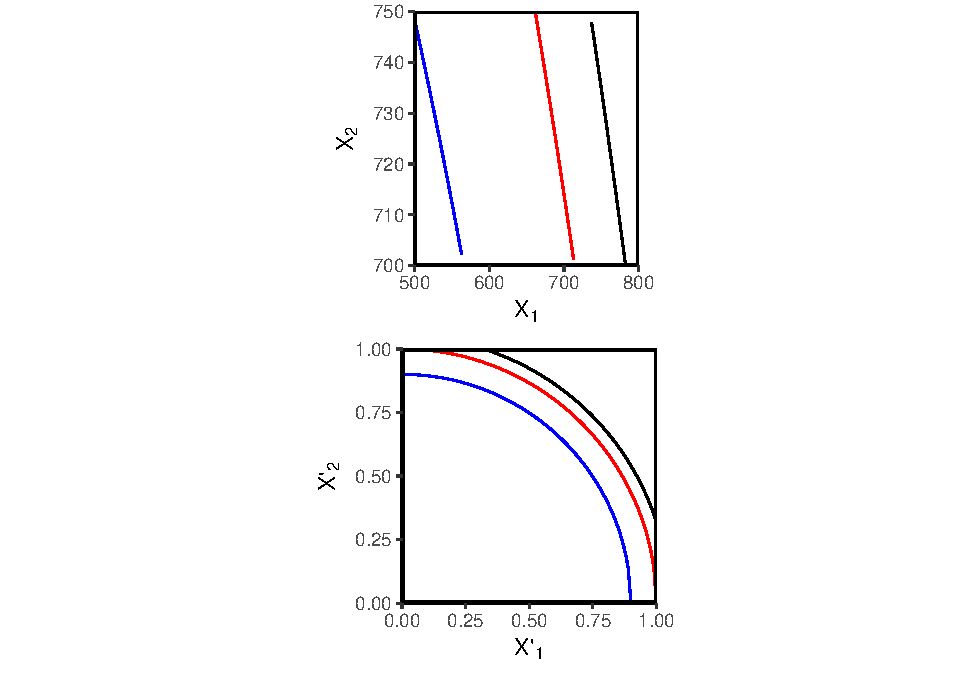
\includegraphics{Trees_with_Base_Functions_files/figure-latex/fig7-curvature-1.pdf}
\caption{\label{fig:fig7-curvature}Behavior of radial IBF with
non-centered/non-scaled variables (top panel) and centered/scaled
variables (bottom panel)}
\end{figure}

\section{5 Benchmarking}\label{benchmarking}

In this section we conduct a benchmarking exercise using a collection of
publicly available datasets that are widely used in the literature to
test the performance of machine learning techniques. The datasets are
listed in Table \ref{tab:Datasets}.

\begin{table}

\caption{\label{tab:dataset-description}\label{tab:Datasets}Datasets for Benchmarking Experiment}
\centering
\resizebox{\linewidth}{!}{
\begin{tabular}[t]{lrrrl}
\toprule
Dataset & Quantitative.Features & Qualitative.Features & Number.of.Cases & Source\\
\midrule
Balance Scale & 4 & 0 & 625 & UCI Machine Learning Repository\\
Wine & 13 & 0 & 178 & Package rattle.data\\
BUPA & 6 & 0 & 345 & Package dprep\\
PIMA Indian & 8 & 0 & 768 & Package mlbench\\
Glass & 9 & 0 & 214 & Package mlbench\\
Book Club & 9 & 1 & 1300 & Package mlbench\\
\bottomrule
\end{tabular}}
\end{table}

As noted above, centering and scaling the variables is important for the
use of IBFs. For the experiments reported in this section, all
quantitative features have been centered on the mean and scaled to the
unit interval. The experiments are using k-fold cross-validation, a
technique commonly used to assess the performance of algorithms that
involves randomly thinning a dataset to obtain a \((100 - 100/k)\)\%
training sample, in a procedure that is repeated \(k\) times. In this
section we use 10-fold cross-validation.

Since one advantage of using IBFs is that they can be used in virtually
any implementation of DTs, we choose to illustrate their broad
applicability using two different methods: a conventional tree algorithm
(as implemented in the R package \texttt{tree}, see Ripley 2018) and an
evolutionary algorithm (as implemented in the package \texttt{evtree},
see Grubinger, Zeileis, and Pfeiffer 2014). Each dataset and method is
used to train trees with oblique partitions and with IBFs. Other R
packages exist that implement non-oblique partitions, however, they are
limited to binary classification (in the \texttt{obliqueRF} package of
Menze and Splitthoff 2012) or to two features (in the spatial oblique
decision trees package \texttt{SPODT} of Gaudart et al. 2015).

In terms of the IBFs, we consider the following functions: \[
\begin{array}{c}\
h_1(b_1(X_1),b_1(X_2))=b_1(X_1)+b_1(X_2)=X_1+X_2\\
h_1(b_2(X_1),b_2(X_2))=b_2(X_1)+b_2(X_2)=X_1^2+X_2^2\\
h_2(b_1(X_1),b_1(X_2))=b_1(X_1)b_2(X_2)=X_1X_2\\
h_2(b_1(X_1)b_3(X_2))=b_1(X_1)b_3(X_2)=X_1e^{X_2}
\end{array}
\]

The size of the experiment is as follows: two different methods
(tree/evolutionary tree), six different datasets, two different types of
partitions (oblique/IBFs), and ten replications for each (i.e., 10-fold
cross-validation).

We report results regarding accuracy, size of the resulting trees, and
computer time. With respect to performance, Figure
\ref{fig:fig8-performance-benchmark-results-train}) shows the accuracy
(in percentage) of the various implementations of the methods. It can be
seen there that introducing IBFs leads at least to comparable
performance, and more often results in performance gains - with the
gains in some cases being quite substantial. This is true regardless of
whether the method is the conventional or evolutionary tree.

\begin{figure}[htbp]
\centering
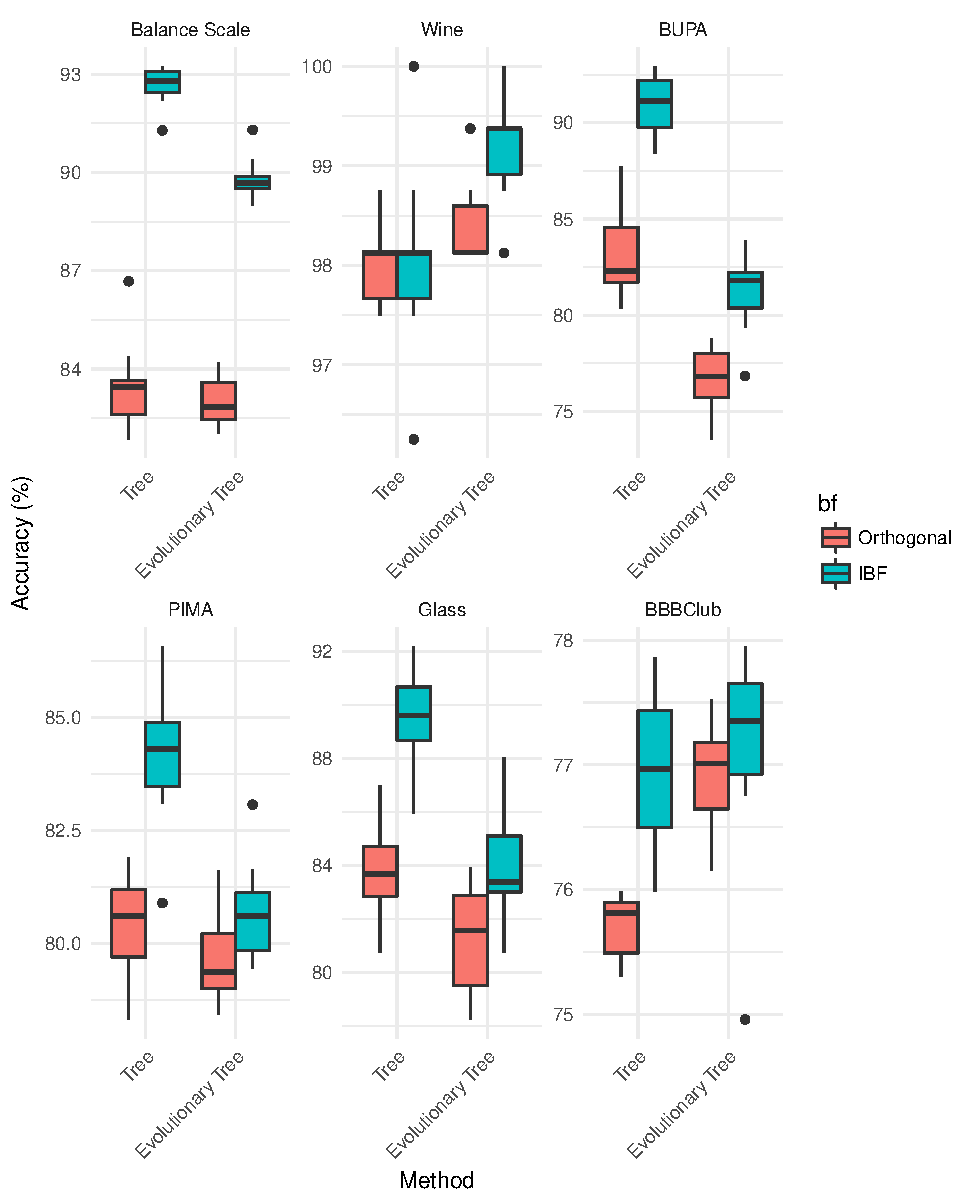
\includegraphics{Trees_with_Base_Functions_files/figure-latex/fig8-performance-benchmark-train-results-1.pdf}
\caption{\label{fig:fig8-performance-benchmark-results-train}Benchmarking
results: Classification accuracy}
\end{figure}

The gains in accuracy do not necessarily imply more complex trees. As
seen in Figure \ref{fig:fig9-performance-benchmark-size-results}, the
\emph{size} of the tree, measured in terms of the number of terminal
nodes, can increase at times (for example, in the case of the BUPA and
PIMA datasets). Other times, the use of IBFs can result in substantial
gains in accuracy simultaneously with a modest reduction in the size of
the tree (as in the case of the Glass dataset).

\begin{figure}[htbp]
\centering
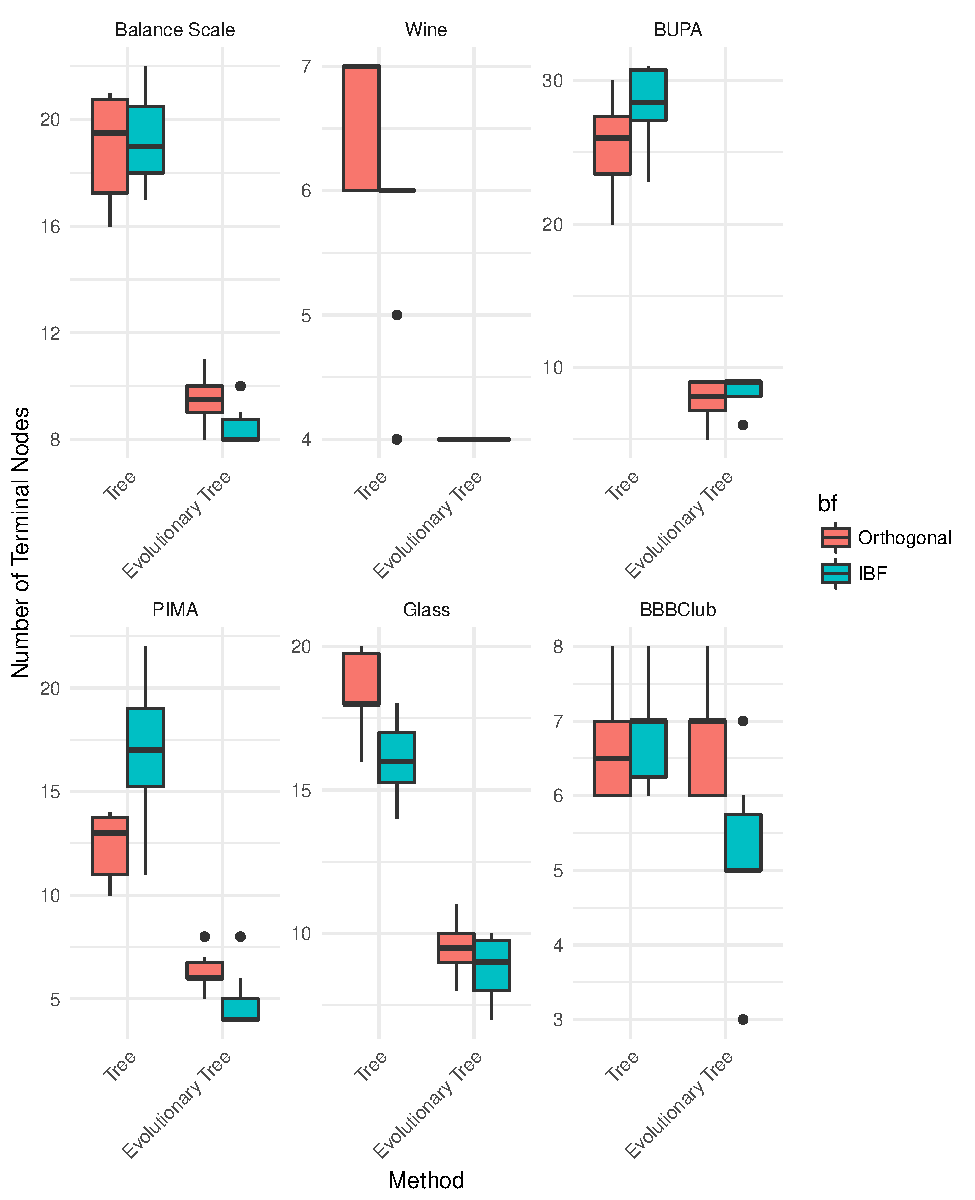
\includegraphics{Trees_with_Base_Functions_files/figure-latex/fig9-performance-benchmark-size-results-1.pdf}
\caption{\label{fig:fig9-performance-benchmark-size-results}Benchmarking
results: Tree size}
\end{figure}

The last result that we report concerns computer time. This part of the
experiment was conducted using the \texttt{microbenchmark} package
(Mersmann 2018). This package times the evaluation of expressions with
sub-millisecond accuracy. Each method/dataset/partition type
(orthogonal, IBF) was evaluated 50 times to produce the results shown in
Figure \ref{fig:fig10-time-benchmark-results}. As seen there, the time
required to train trees with IBFs is comparable or occasionally somewhat
more favorable than with oblique partitions, perhaps as a consequence of
finding better partitions in fewer dimensions.

\begin{figure}[htbp]
\centering
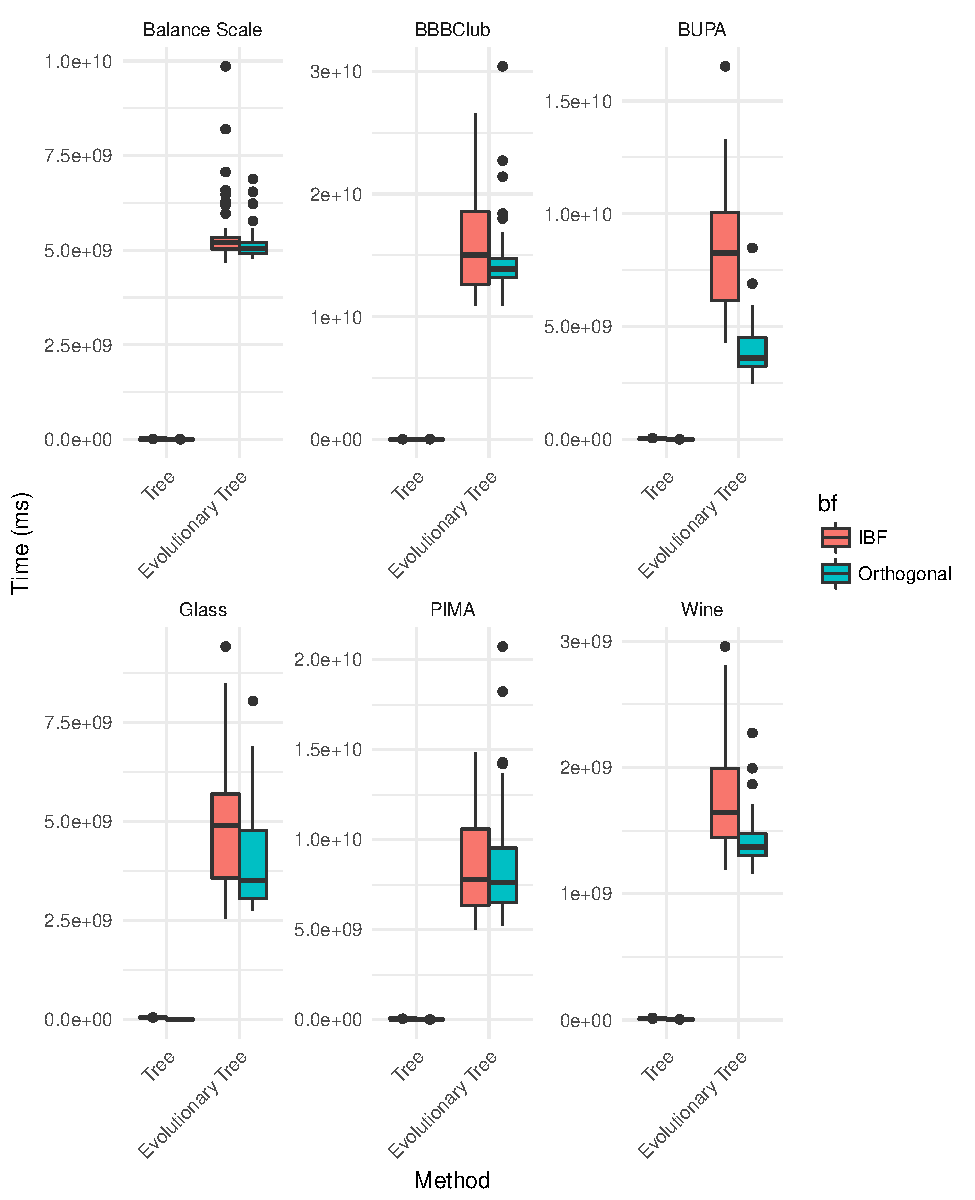
\includegraphics{Trees_with_Base_Functions_files/figure-latex/fig10-time-benchmark-results-1.pdf}
\caption{\label{fig:fig10-time-benchmark-results}Benchmarking results:
Computing time}
\end{figure}

\section{6 Sample Applications}\label{sample-applications}

As illustrated in the benchmarking exercise above, the modelling
strategy proposed here works well on multifeature datasets. Furthermore,
inducing oblique and/or non-linear partitions can improve the
performance of DTs. In this section, we complement the results of the
benchmarking experiment by presenting three empirical examples. One of
these examples is a classification problem, and two examples are
regressions on quantitative variables. Two of the examples are of
geographical interest and have the advantage that the features are
geospatial, which greatly facilitates the visualization of the results.
The third example is a multifeature set. In this case, we solve the
issue of visualizing non-oblique partitions by means of a device that we
call \emph{decision charts}.

\subsection{6.1 Classification Example: Ethnic
Neighborhoods}\label{classification-example-ethnic-neighborhoods}

The first example that we present is concerned with a spatial
classification problem. This kind of problem is often found in
geography, public health, and sociology, among other disciplines, and
addresses the objective of defining spatial neighborhoods. Examples of
this kind of research in the literature include include Gaudart et al.
(2005), a team of reserchers who developed oblique DTs to identify high
risk clusters of malaria. Research by Folch and Spielmann (2014) led to
an algorithm to identify regions with flexible constraints. Wong and
Huang (2017) identify geographical spheres of influence based on social
media data. One more example is the research by Logan et al. (2011) that
aimed at identifying ethnic neighborhoods using historical datasets.

The example presented here is similar in spirit to the research of Logan
et al. (2011), and makes use of a portion of the same historical dataset
(see John R. Logan et al. 2011). The dataset consists of 21520
individual records for part of Newark, coded by ethnicity according to
the 1880 US Census. Of these, 7,659 records are classified as White
Americans, 4,411 are classified as Irish, and 9,450 are classified as
German. The geographical distribution of these groups in the region of
Newark under study is shown in Figure \ref{fig:fig11-map-newark}.

\begin{figure}[htbp]
\centering
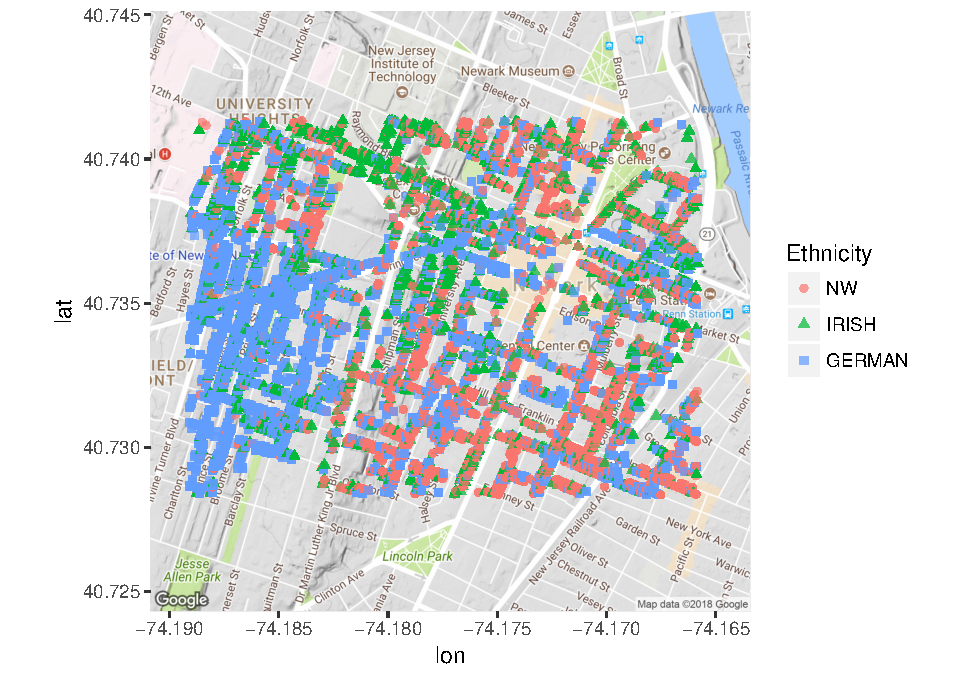
\includegraphics{Trees_with_Base_Functions_files/figure-latex/fig11-map-newark-1.pdf}
\caption{\label{fig:fig11-map-newark}Three ethnic groups in Newark (1880
US Census)}
\end{figure}

Since the objective of the example is to find homogeneous neighborhoods,
this examples considers only two features, namely the coordinates of the
observations in longitude and latitude. The following IBFs are
introduced as additional features: \[
\begin{array}{c}\
h_1(b_1(long),b_1(lat))=b_1(long)+b_1(lat)=long+lat\\
h_2(b_1(long),b_1(lat))=b_1(long)b_1(lat)=long\times lat\\
h_1(b_2(long),b_2(lat))=b_2(long)+b_2(lat)=long^2+lat^2\\
h_1(b_3(long),b_3(lat))=b_3(long)+b_3(lat)=e^{long}+e^{lat}\\
h_2(b_3(long)b_3(lat))=b_3(long)b_3(lat)=e^{long}\times e^{lat}
\end{array}
\]

After some experimentation, the coordinates of the observations were
centered at the top right corner of the set of points, and scaled to the
unit on the longest extent of the dataset. For comparison purposes, we
begin by training a DT for this problem using conventional orthogonal
partitions. The results of this model are shown in Figure
\ref{fig:fig12-tree-orthogonal-newark}, a model with six terminal nodes
that identify two predominantly German neighborhoods, three
predominantly White American neighborhoods, and one predominantly Irish
neighborhood. The model, after examining the interior branches, did not
require pruning.

This model has an in-sample error rate of 0.39 and a cross-validation
error rate of 0.39. The population of two of the White American
Neighborhoods is over 60\% of that ethnic group. Another neighborhood
has a plurality (49\%) of White Americans and a more or less even
distribution of Irish (22\%) and Germans (29\%). One neighborhood is
strongly Irish (62\% of population) with White American and German
minorities (27\% and 11\% respectively). Another neighborhood is
strongly German, with over 70\% of the residents of that ethnicity,
whereas one more has a plurality of Germans (41\%) but is otherwise
quite mixed. The partitions of the DT in effect delimit the ethnic
neighborhoods, as seen Figure \ref{fig:fig13-map-orthogonal-newark}.

\begin{figure}[htbp]
\centering
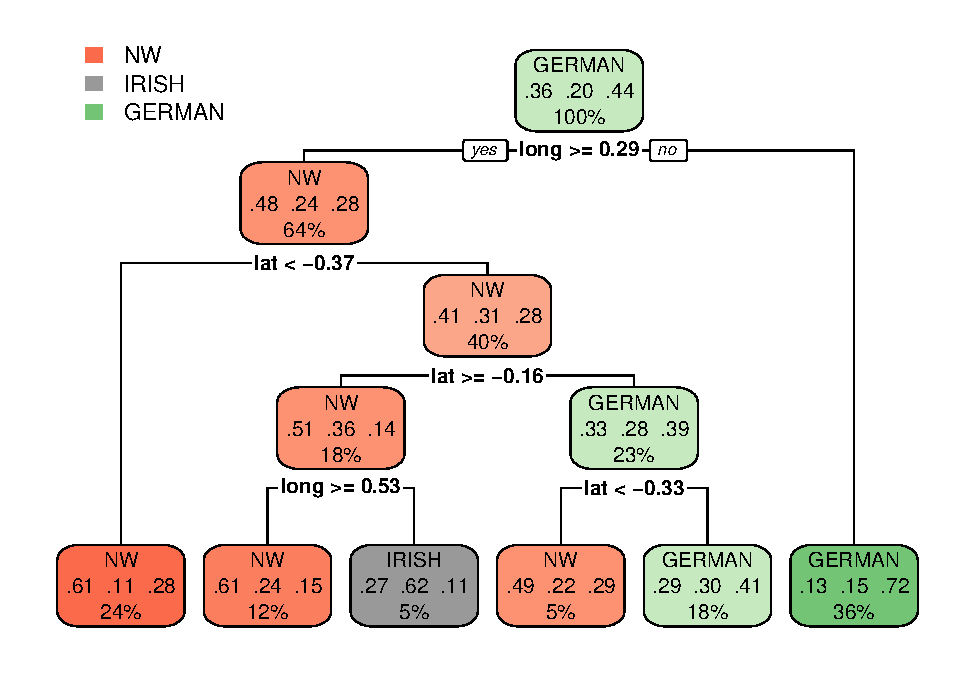
\includegraphics{Trees_with_Base_Functions_files/figure-latex/fig12-tree-orthogonal-newark-1.pdf}
\caption{\label{fig:fig12-tree-orthogonal-newark}Decisiton tree with
orthogonal partitions for spatial classification, Newark ethnic groups}
\end{figure}

\begin{figure}[htbp]
\centering
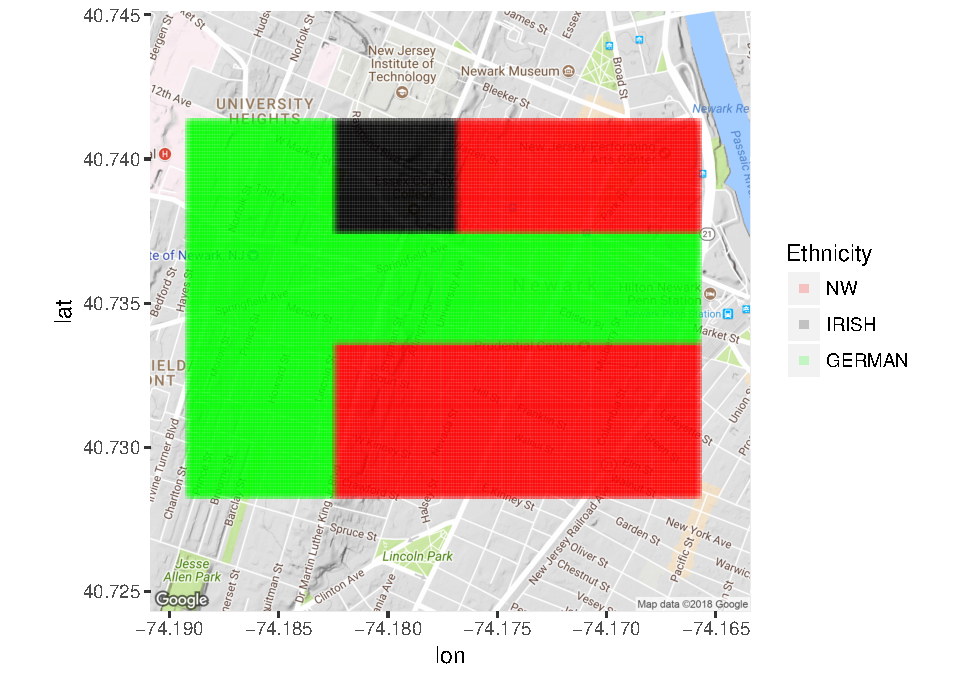
\includegraphics{Trees_with_Base_Functions_files/figure-latex/fig13-map-orthogonal-newark-1.pdf}
\caption{\label{fig:fig13-map-orthogonal-newark}Ethnic neighborhoods in
Newark, 1880, using orthogonal partitions}
\end{figure}

Next, the same dataset is used to train a tree with IBFs as listed
above. The model was examined to determine that pruning was not
required. The results of this model are shown in Figure
\ref{fig:fig14-tree-basis-newark}. The model also has six terminal nodes
which identify two German neighborhoods, three White American
neigborhoods, and one Irish neighborhoods. Note that two of the
partitions are orthogonal (i.e., \(lat < -0.37\) and \(lat \ge -0.16\)),
two partitions are linear but oblique (i.e., \(long+lat \ge 0.51\) and
\(long+lat \ge 0.21\)), and one partition is non-linear (i.e.,
\(e^{long}+e^{lat} \ge 2.0\)). The ethnic neighborhoods are shown in
Figure \ref{fig:fig15-map-basis-newark}. This model has an in-sample
error rate of 0.39 and a cross-validation error rate of 0.39, which is
comparable to the orthogonal model. In this case, the analyst must
decide whether the neighborhoods identified by the DT with IBFs are a
more realistic representation of a spatial process.

\begin{figure}[htbp]
\centering
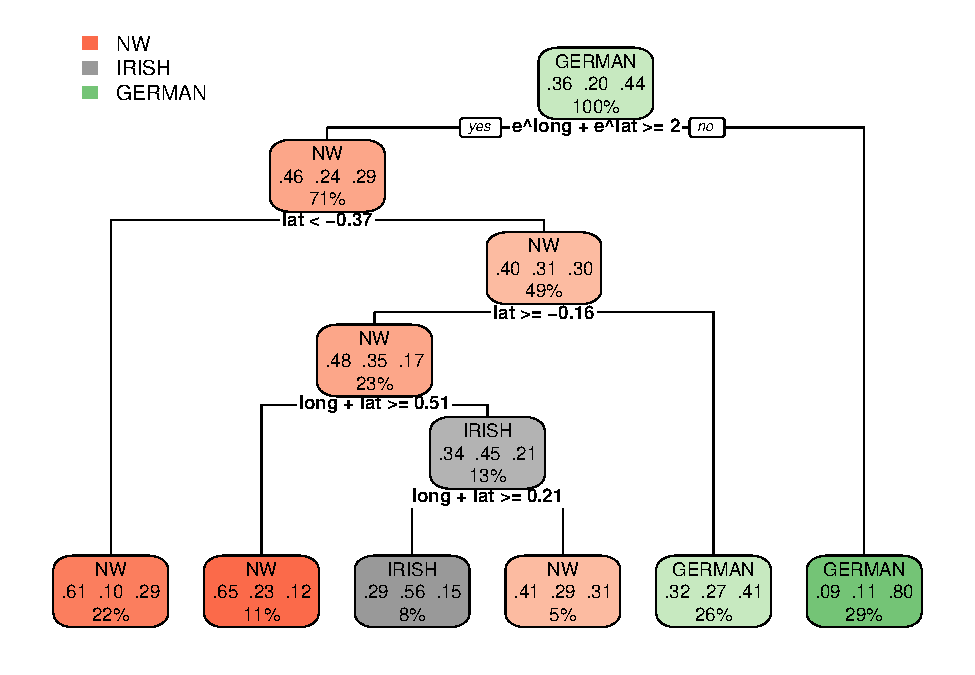
\includegraphics{Trees_with_Base_Functions_files/figure-latex/fig14-tree-basis-newark-1.pdf}
\caption{\label{fig:fig14-tree-basis-newark}Decision tree with
non-orthogonal/non-linear partitions for spatial classification, Newark
ethnic groups}
\end{figure}

\begin{figure}[htbp]
\centering
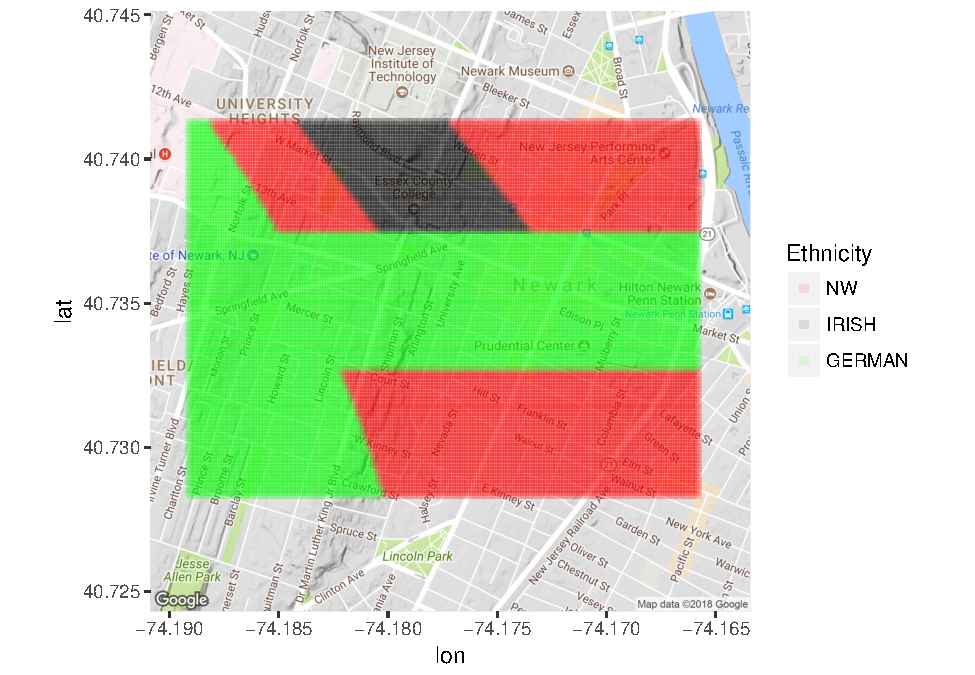
\includegraphics{Trees_with_Base_Functions_files/figure-latex/fig15-map-basis-newark-1.pdf}
\caption{\label{fig:fig15-map-basis-newark}Ethnic neighborhoods in
Newark, 1880, using non-orthogonal partitions}
\end{figure}

\subsection{6.2 Regression Example: Spatial Market
Segmentation}\label{regression-example-spatial-market-segmentation}

The case presented next is similar to the spatial classification problem
above, except that it is now a regression situation. The example relates
to an issue widely discussed in the real estate and property valuation
literature, and is concerned with the identification of spatial
submarkets. Numerous papers exist on this topic, including Gabriel
(1984), Feitelson (1993), Paez et al. (2001), Bourassa et al. (2003),
Helbich et al. (2013), and Wheeler et al. (2014). More recently, DTs
have been applied to identify spatial market segments in a real estate
setting by Fuss and Koller (2016), however using orthogonal partitions.

One obvious limitation of using orthogonal partitions in the case of
real estate spatial submarkets is that the processes that drive land
rent (and therefore property values) tend to be radial and are possibly
anisotropic due to inhomogeneities in the landscape. The canonical urban
economic theory for monocentric cities (which has since been expanded to
polycentric cities) states that land rent decays from business districts
(Alonso 1964), a prediction that is borne by numerous empirical studies.

The illustration presented here deals with land prices in Sapporo,
Japan. The dataset consists of 429 observations of geocoded land prices
(in \(\yen/m^2\)). Informed by the literature on property valuation, the
coordinates (in longitude and latitude) were centered on the geometric
mean of the locations of the observations, a location that coincides
with the central business district of the city. Further, the coordinates
were scaled to the unit on the longest extent of the dataset. Land
prices were log-transformed to mitigate their lack of normality. Figure
\ref{fig:fig16-map-sapporo} shows the locations of the observations and
prices. As can be seen there, Sapporo is a typical monocentric city,
with the highest prices concentrated in and around the central business
district.

\begin{figure}[htbp]
\centering
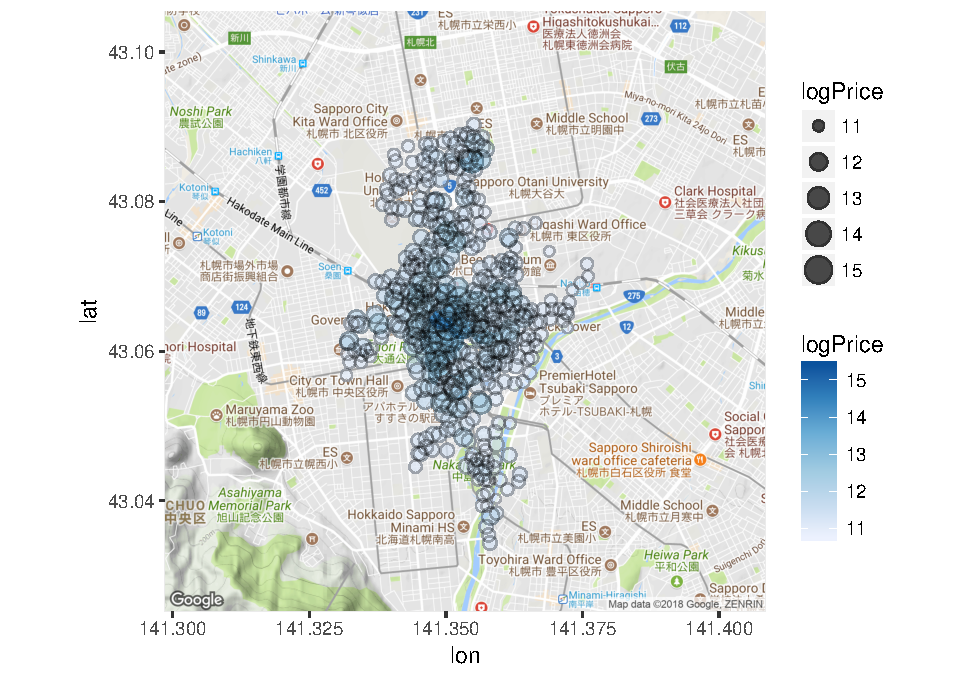
\includegraphics{Trees_with_Base_Functions_files/figure-latex/fig16-map-sapporo-1.pdf}
\caption{\label{fig:fig16-map-sapporo}Land prices in Sapporo (log)}
\end{figure}

As before, we train a DT using orthogonal partitions. The results of
this model are shown in Figure \ref{fig:fig17-tree-orthogonal-sapporo},
where it can be seen that the tree has thirteen terminal nodes, or
equivalently spatial submarkets. This was the best-performing tree size,
and there was no need to prune. The \(pseudo-R^2\) of this model is
\(0.71\). The submarkets are shown in Figure
\ref{fig:fig18-map-orthogonal-sapporo}, where it can be seen that the
submarkets manage to capture the monocentric structure of land prices in
Sapporo, albeit in cubist style.

\begin{figure}[htbp]
\centering
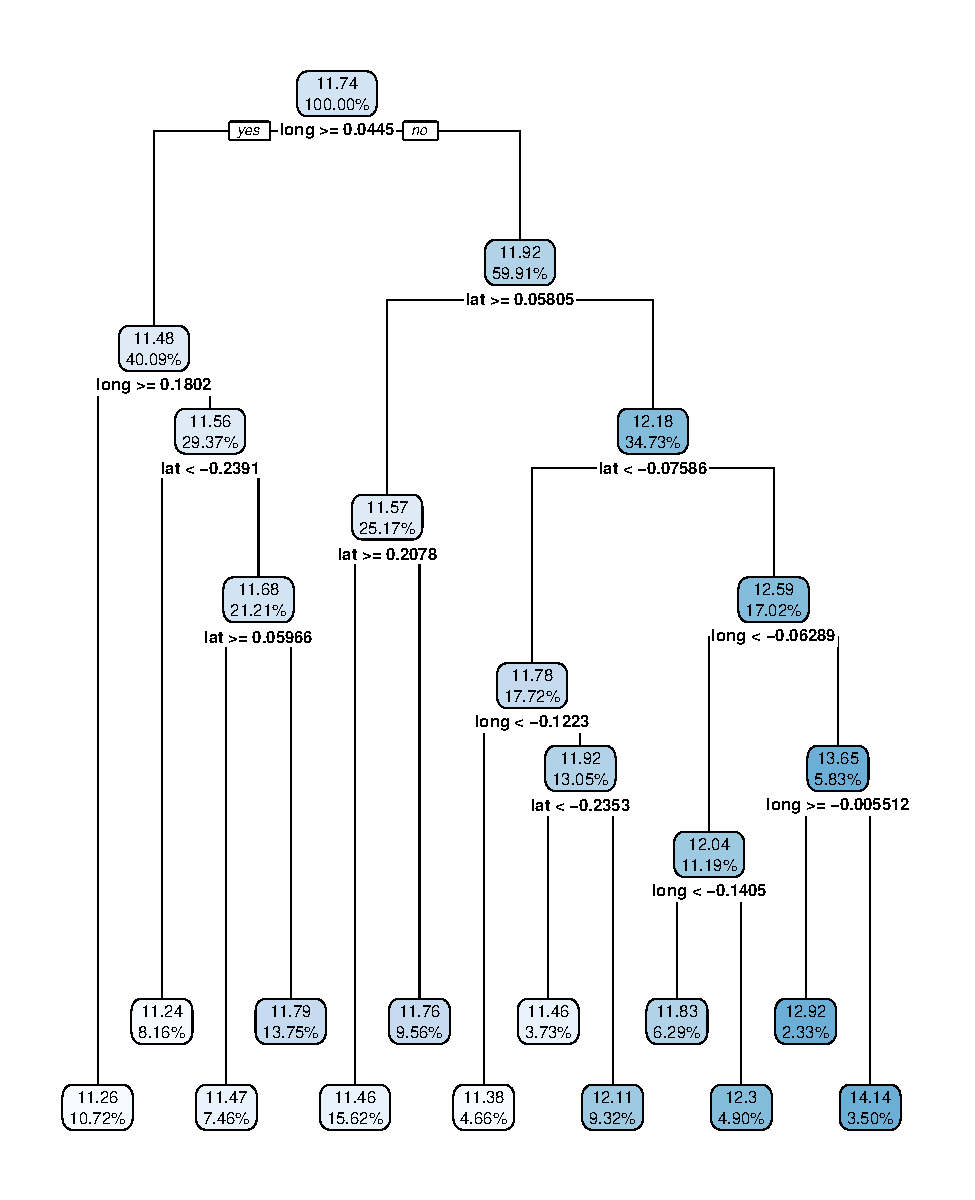
\includegraphics{Trees_with_Base_Functions_files/figure-latex/fig17-tree-orthogonal-sapporo-1.pdf}
\caption{\label{fig:fig17-tree-orthogonal-sapporo}Decision tree with
orthogonal partitions for submarket identification, Sapporo land prices}
\end{figure}

\begin{figure}[htbp]
\centering
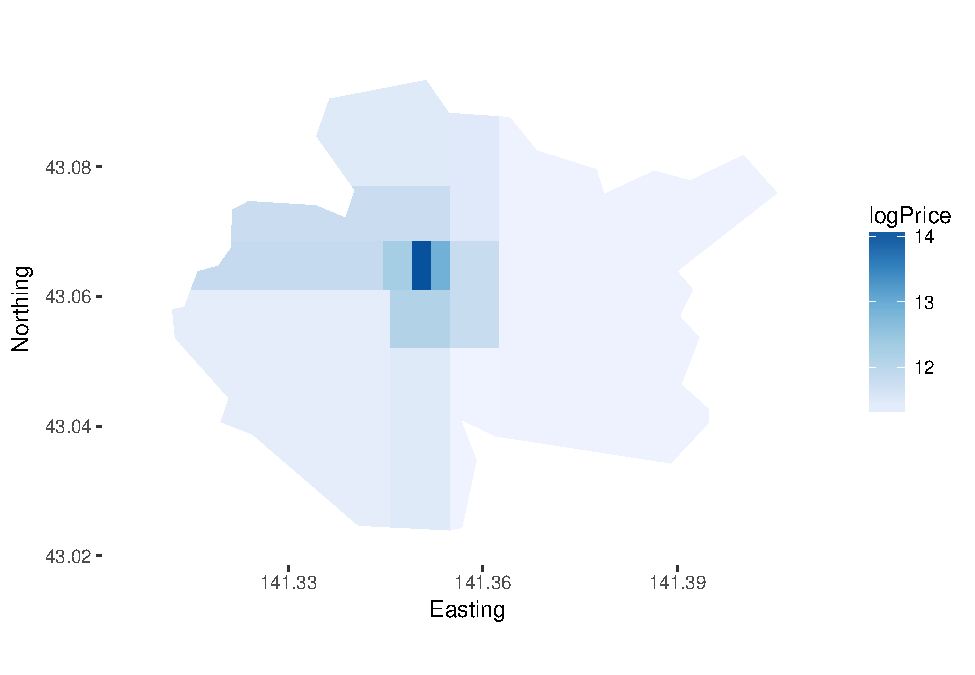
\includegraphics{Trees_with_Base_Functions_files/figure-latex/fig18-map-orthogonal-sapporo-1.pdf}
\caption{\label{fig:fig18-map-orthogonal-sapporo}Spatial land price
submarkets in Sapporo using orthogonal partitions}
\end{figure}

The next step was to train a DT, but this time using IBFs as additional
features in the dataset. The basis functions used are the same five IBFs
used in the preceding example. The resulting DT was checked to see if
pruning was appropriate, but the full tree gave the best results (see
Figure \ref{fig:fig19-tree-basis-sapporo}). It is worthwhile noting that
only one of seven partitions is orthogonal. The remaining six partitions
are all non-linear. The number of terminal nodes/submarkets is eight
compared to thirteen in the model with orthogonal partitions. Both
models have a comparable performace, with a \(pseudo-R^2=0.71\), however
the use of IBFs results in a more parsimonious model. Furthermore, the
resulting market segments (see Figure \ref{fig:fig20-map-basis-sapporo})
are much more appealing, and conform better to our theoretical
understanding of the radial and anisotropic mechanisms of land price
determination.

\begin{figure}[htbp]
\centering
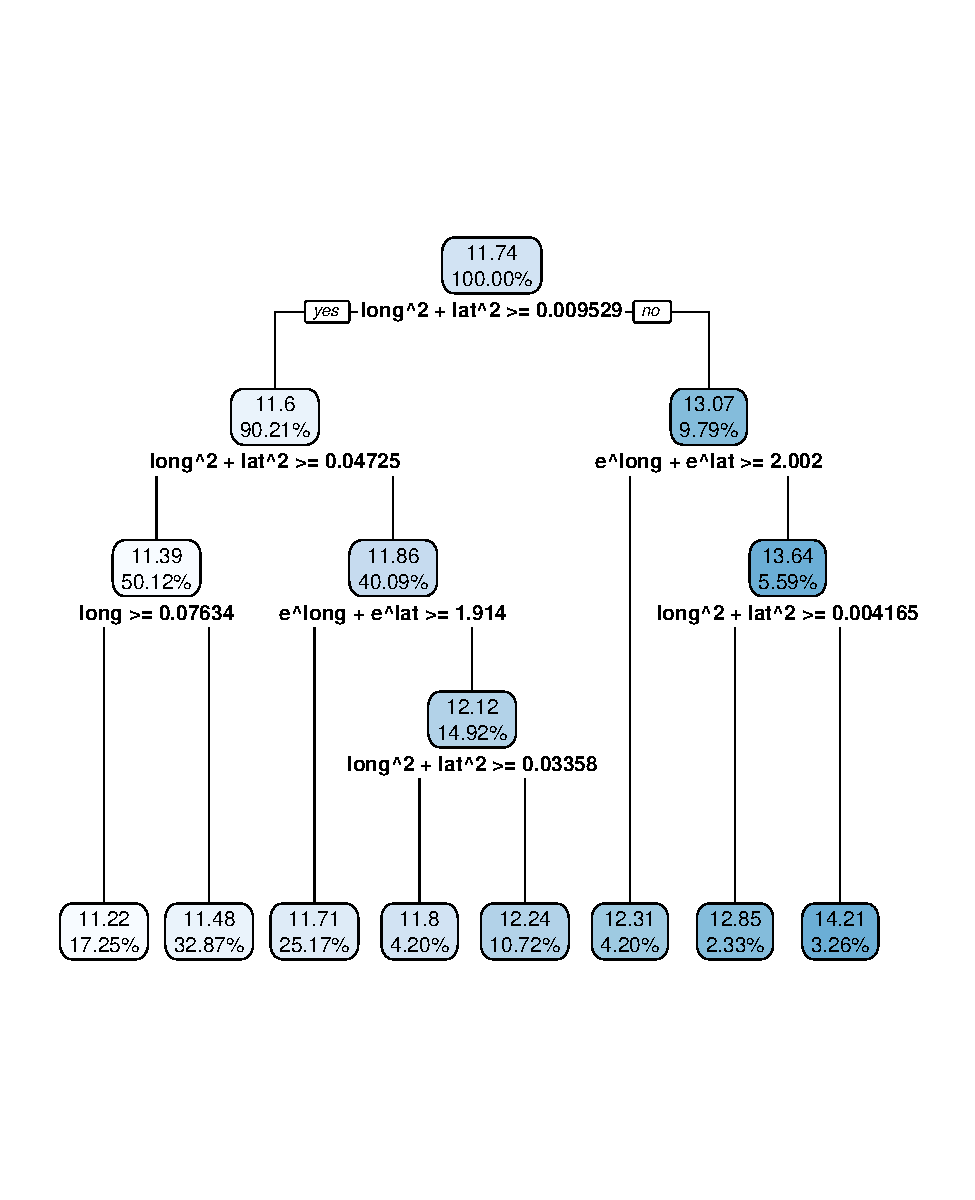
\includegraphics{Trees_with_Base_Functions_files/figure-latex/fig19-tree-basis-sapporo-1.pdf}
\caption{\label{fig:fig19-tree-basis-sapporo}Decision tree with
non-orthogonal/non-linear partitions for submarket identification,
Sapporo land prices}
\end{figure}

\begin{figure}[htbp]
\centering
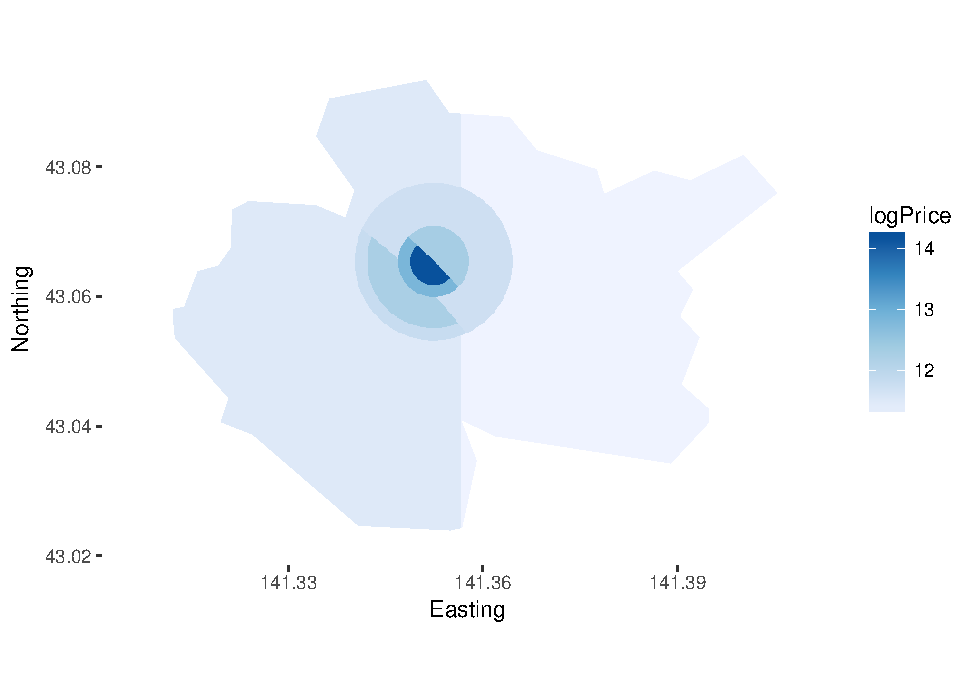
\includegraphics{Trees_with_Base_Functions_files/figure-latex/fig20-map-basis-sapporo-1.pdf}
\caption{\label{fig:fig20-map-basis-sapporo}IBF-based non-orthogonal
land price regions (log) in Sapporo}
\end{figure}

\subsection{6.3 Regression Example: Voter
Turnout}\label{regression-example-voter-turnout}

The previous two examples were of DTs trained using only two features
(the coordinates of the observations) and augmented by means of IBFs.
Both examples dealt with forms of spatial segmentation which
incidentally facilitate the visualization of the non-orthogonal and
non-linear partitions that result from the use of IBFs. In the last
example the we present, we use a multifeature dataset of voter turnout
in a recent provincial election in Ontario, Canada.

Voter turnout is an issue of interest to behavioral and political
scientists, who identify this aspect of democracies as one of three key
indicators of their performance (Powell 1982). Moreover, voter turnout
tends to vary quite substantially by region, a fact that has motivated a
voluminous literature (starting with the pioneering research of Powell
1982; Powell 1986; and Jackman 1987) that aims at understanding the
factors that correlate with voter turnout. Numerous studies exist that
empirically test the relationships between voter turnout and a variety
of socio-economic, demographic, and other variables (for a relevant
review see Geys 2006; and more recently Stockemer 2017).

The case presented in this section is of the 2018 provincial election in
Ontario, Canada. Data were obtained from three sources. First, a
geography file of Electoral Districts in Ontario was obtained from
Elections Ontario
(https://www.elections.on.ca/en/voting-in-ontario/electoral-district-shapefiles/limited-use-data-product-licence-agreement/download-shapefiles.html).
The effectively final counts of the election were obtained from a
political blog and cross-checked with information from Elections Ontario
for accuracy
(https://quandyfactory.com/blog/201/unofficial\_ontario\_2018\_election\_riding\_by\_riding\_summary\_table).
Finally, socio-economic and demographic information was retrieved from
the 2016 Canadian Census. Census data were obtained at the level of
Census Subdivisions. Electoral Districts are sometimes larger than
Census Subdivisions, so census variables were converted to the Electoral
Districts by aggregation in the case of absolute values (e.g.,
population, population by educational achievement), or by calculating
their area-weighted averages in the case of rates (e.g., median income).

The dataset consists of 124 records (one for each electoral district),
and seventeen variables, with descriptive statistics as shown in Table
\ref{tab:descriptive-statistics-election}. Voter turnout is calculated
as the proportion of total votes to number of registered electors. The
selection of variables reflects an interest in geographical context
(e.g., population density and median commute duration), the effect of
government policy (\% of government transfers relative to income and
average income taxes as percent of income), in addition to features
relating to age, income, poverty, and academic achievement. These
variables were centered on their minimum values and scaled to the unit
interval prior to the analysis.

\begin{table}

\caption{\label{tab:descriptive-statistics-election}\label{tab:descriptive-statistics-election}Descriptive statistics for electoral districts in Ontario, 2018}
\centering
\resizebox{\linewidth}{!}{
\begin{tabular}[t]{llllll}
\toprule
Variable & Abbv & Min & Max & Mean & std\\
\midrule
Voter\_Turnout & Turnout & 0.44 & 0.67 & 0.58 & 0.047\\
Pop\_Den & PD & 0.091 & 4150 & 1349 & 1567\\
Median\_Age & MA & 12 & 51 & 39 & 4.9\\
Median\_Income & MI & 11776 & 40831 & 29901 & 5275\\
Male\_Median\_Income & MMI & 12972 & 51442 & 36029 & 6960\\
\addlinespace
Female\_Median\_Income & FMI & 10478 & 33728 & 25042 & 4193\\
Pct\_Government\_Transfer\_Payments & PGTP & 6.1 & 23 & 13 & 3.6\\
Median\_Commute\_Dur & MCD & 7.3 & 35 & 23 & 6.6\\
Avg\_Inc\_Taxes\_as\_Pct\_Inc & AITPI & 3.8 & 24 & 16 & 3.4\\
Pct\_Population\_in\_Low\_Income & PPLI & 1.8 & 24 & 13 & 4.5\\
\addlinespace
Prop\_no\_certificate & PNC & 0.044 & 0.29 & 0.11 & 0.036\\
Prop\_HS\_diploma & PHSD & 0.17 & 0.32 & 0.24 & 0.04\\
Prop\_Post\_HS\_diploma & PPHSD & 0.49 & 0.79 & 0.64 & 0.067\\
Prop\_trade\_certificate & PTC & 0.043 & 0.15 & 0.08 & 0.027\\
Prop\_college\_diploma & PCD & 0.17 & 0.33 & 0.24 & 0.045\\
\addlinespace
Prop\_university\_bachelor & PUB & 0.068 & 0.29 & 0.17 & 0.065\\
Prop\_postgraduate & PPG & 0.029 & 0.19 & 0.11 & 0.048\\
\bottomrule
\end{tabular}}
\end{table}

We started by training an initial DT which resulted in a model with
eleven terminal nodes. This model was examined, and based on performance
was eventually pruned to give the model shown in Figure
\ref{fig:fig21-tree-orthogonal-election}. This model has a
\(pseudo-R^2\) of \(0.24\). As seen in the figure, the model is
relatively simple, and identifies two covariates that correlate with
voter turnout, namely \% of population living in low income and
population density. The lowest voter turnout rates are associated with
Electoral Districts with higher rates of population living in poverty,
whereas the highest turnout rates are associated with Electoral
Districts characterized by higher population density and low poverty
rates.

\begin{figure}[htbp]
\centering
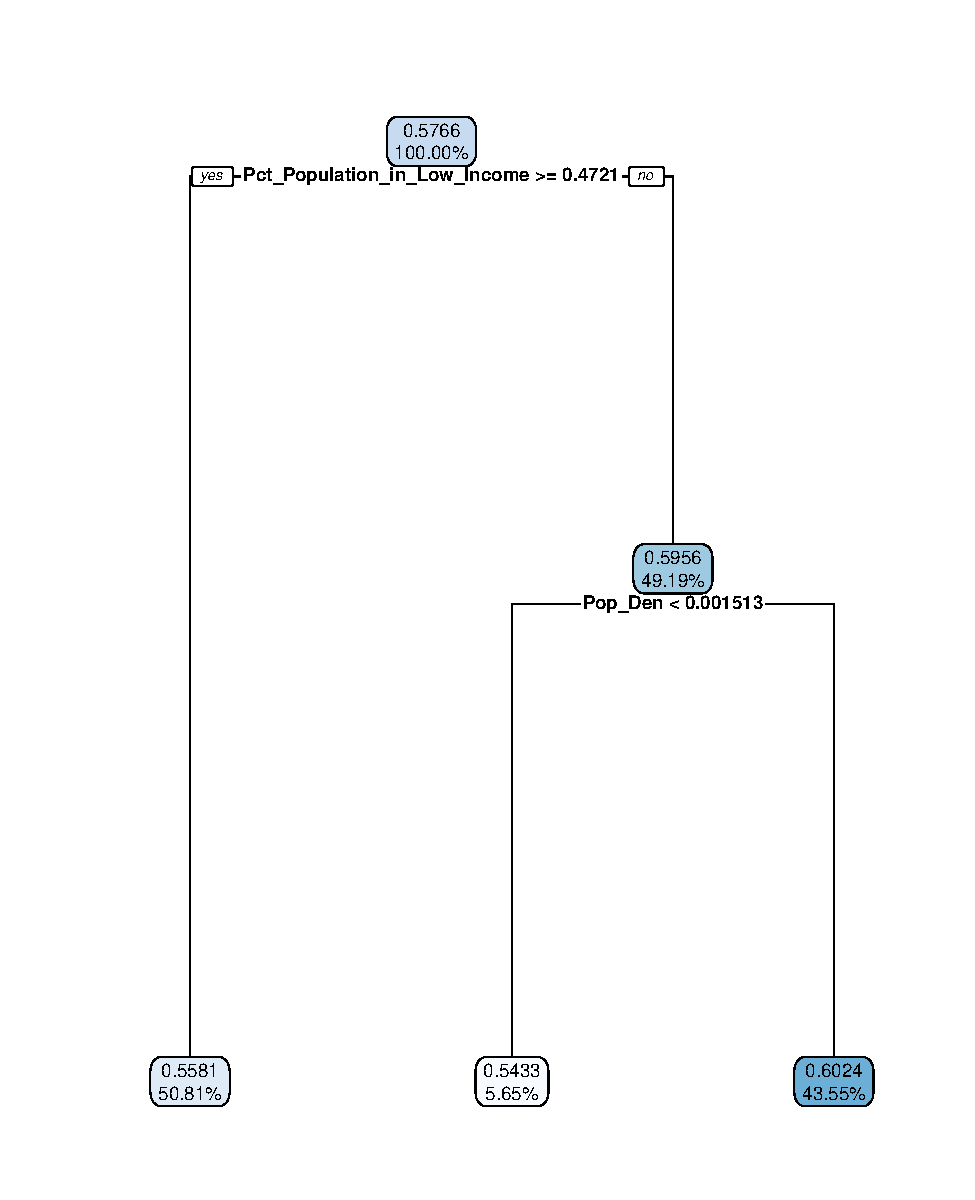
\includegraphics{Trees_with_Base_Functions_files/figure-latex/fig21-tree-orthogonal-election-1.pdf}
\caption{\label{fig:fig21-tree-orthogonal-election}Decision tree with
orthogonal partitions, Ontario voter turnout}
\end{figure}

The next step was to train a model that included IBFs as above. The
initial model had eleven terminal nodes, but upon examination was pruned
to produce the model shown in Figure
\ref{fig:fig22-tree-basis-election}. The \(pseudo-R^2\) of this model is
\(0.44\). Note that three of the partitions in this model are oblique,
and one is non-linear. Population density (PD), which appeared in the
model with orthogonal partitions, is still part of this model in the
last interior node. However, percentage of population living in poverty
is not. Instead, average income taxes as percentage of income (AITPI),
median age (MA), and several academic achievement variables entered the
model (proportion of trade certificates: PTC; proportion of college
diploma: PCD; proportion of high school diploma: PHSD; proportion of
university bachelor: PUB; and propotion with no certificate: PNC). These
variables are often correlated with population living in poverty, but
give a more refined view of the characteristics of populations that
associate with voter turnout.

\begin{figure}[htbp]
\centering
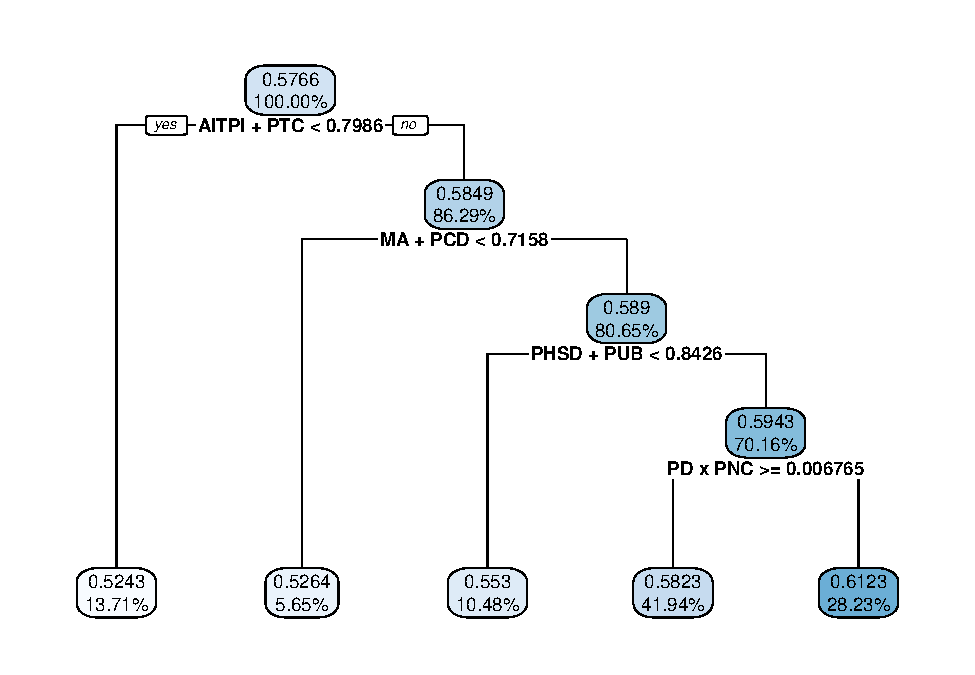
\includegraphics{Trees_with_Base_Functions_files/figure-latex/fig22-tree-basis-election-1.pdf}
\caption{\label{fig:fig22-tree-basis-election}Decision tree with
non-orthogonal/non-linear partitions, Ontario voter turnout}
\end{figure}

In the case of a multifeature dataset, interpretation of a DT with IBFs
is not as straightforward as it was for orthogonal partitions,
particularly considering that the variables were centered and scaled. In
order to enhance the interpretability of the results of models with
IBFs, we propose to use a device we call decision charts. These charts
allow us to plot the decision boundaries in the space of the two basis
implied by each node of the tree. By recentering and rescaling the
decision boundaries back to the units of the original basis vectors, a
simple protocol can be devised to interpret the results of a model. The
maps in the previous two examples showing ethnic boundaries and market
segments are essentially decision charts for the case of two features.
An example of a set of decision charts for the multifeature voter
turnout model is shown in Figure
\ref{fig:fig23-election-decision-charts}.

\begin{figure}[htbp]
\centering
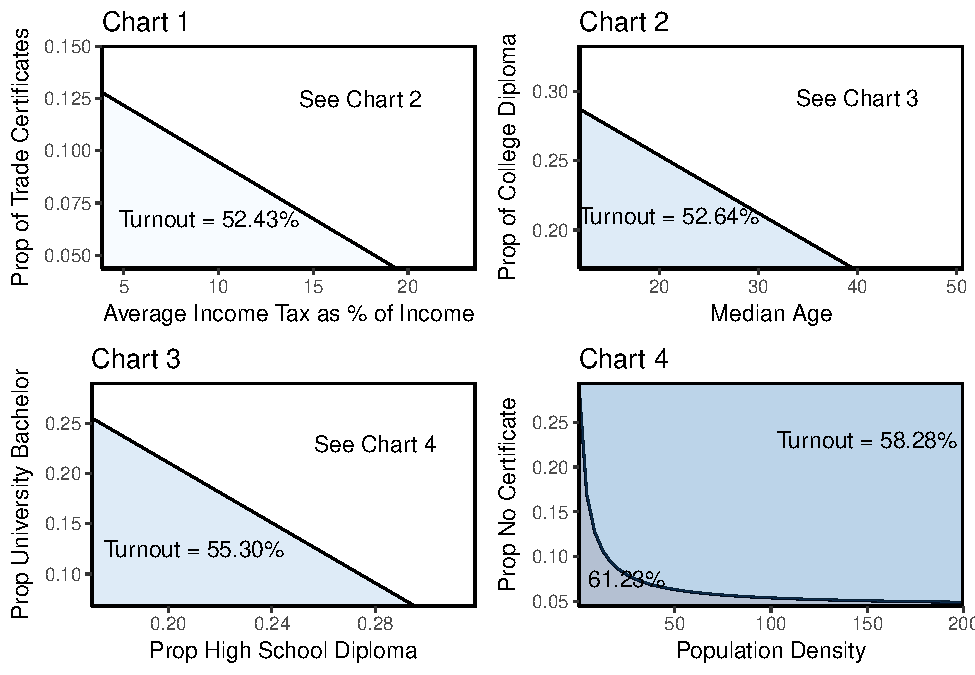
\includegraphics{Trees_with_Base_Functions_files/figure-latex/fig23-election-decision-charts-1.pdf}
\caption{\label{fig:fig23-election-decision-charts}Decision charts for
voter turnout}
\end{figure}

As seen in the figure, low voter turnouts are associated with Electoral
Districts where income taxes as percentage of income are on average low,
and that \emph{simultaneously} have relatively high proportions of
residents with trade certificates (an indication of the presence of blue
collar workers). High voter turnout rates, in contrast, are associated
with Electoral Districts that tend to be older and better educated (tops
of Charts 2 and 3), and with high population density \emph{or} low
population density and a high proportion of people without certificate
(bottom of Chart 4).

\section{7 Conclusions and Directions for Future
Research}\label{conclusions-and-directions-for-future-research}

Decision Trees are a popular data analysis technique used in a wide
range of applications. The somewhat restrictive nature of binary
orthogonal partitions has been recognized in the past, and a number of
methods have been proposed in the literature to allow for oblique
partitions. In this paper, we have proposed a new strategy to induce
oblique and non-linear partitions for DTs. This is achieved by
introducing Interactive Basis Functions. The use of IBFs is attractive
because it can induce partitions of different shapes at a relatively low
computational cost. Furthermore, the underlying recursive-partition
algorithm is not changed, which means that IBFs can be used with any
implementation of DTs in existing software.

A benchmarking exercise shows that the use of IBFs can improve the
accuracy of the model and/or produce more parsimonious models, without
greatly increasing computation time. Furthermore, three case studies
illustrated the application and potential advantages of IBFs. In one
spatial classification example, the accuracy of the model was maintained
but potentially more appealing boundaries were identified. In a market
segmentation example, likewise, accuracy was maintained but a more
parsimonious and theoretically consistent model was obtained. And in a
multifeature model of voter turnout, IBFs led to a better model fit and
a more parsimonious model.

One downside of using oblique/non-linear partitions in DTs is that the
interpretability of the typical visual output (as a tree with binary
branches) becomes compromised. To remedy this situation we introduced a
new tool called decision charts, a set of visual devices where new
inputs can be located to help an analyst to reach a decision using the
underlying DT.

As we noted in the paper, the additive IBF is equivalent to previous
efforts to induce oblique partitions, with a key simplification: the
assumption that the function is non-parametric. Obviously,
parameterizing an IBF could increase its flexibility, however at a
higher computational cost. Whether this higher computational cost
exceeds that of, say, the CART-LC method, is an open question. A
research challenge would be to parameterize other IBFs for increasingly
flexible non-linear partitions. Finally, a limitation of the development
presented in this paper is that it only applies to quantitatie features,
and therefore it would be interesting to explore possible extensions for
qualitative features. This is also a matter for future research.

\section{Acknowledgments}\label{acknowledgments}

F.A. Lopez, M. Ruiz and M. Camacho acknowledge the financial support
from projects ECO2015-65758-P, ECO2015-65637-P, and ECO2016-76178-P
respectively. This study is the result of the activity carried out under
the program Groups of Excellence of the Region of Murcia, the Fundacion
Seneca, Science and Technology Agency of the region of Murcia project
19884/GERM/15. The following R packages were used during this research,
and the authors wish to acknowledge their developers: \texttt{tidyverse}
(Wickham 2017), \texttt{plyr} (Wickham 2011), \texttt{readxl} (Wickham
and Bryan 2018), \texttt{ggthemes} (Arnold 2018), \texttt{tree} (Ripley
2018), \texttt{evtree} (Grubinger, Zeileis, and Pfeiffer 2014),
\texttt{rpart} (Therneau, Atkinson, and Ripley 2017),
\texttt{rpart.plot} (Milborrow 2018), \texttt{ggmap} (Kahle and Wickham
2013), \texttt{readr} (Wickham, Hester, and Francois 2017),
\texttt{rgdal} (Bivand, Keitt, and Rowlingson 2018), \texttt{knitr} (Xie
2015; Xie 2018), \texttt{kableExtra} (Zhu 2018), \texttt{mlbench}
(Newman et al. 1998), \texttt{dprep} (Acuna and CASTLE research group at
The University of Puerto Rico-Mayaguez 2015), \texttt{rattle.data}
(Williams 2011), \texttt{microbenchmark} (Mersmann 2018),
\texttt{RColorBrewer} (Neuwirth 2014), \texttt{scales} (Wickham 2018),
and \texttt{gridExtra} (Auguie 2017).

\section*{References}\label{references}
\addcontentsline{toc}{section}{References}

\hypertarget{refs}{}
\hypertarget{ref-Acuna2015}{}
Acuna, Edgar, and the CASTLE research group at The University of Puerto
Rico-Mayaguez. 2015. \emph{Dprep: Data Pre-Processing and Visualization
Functions for Classification}.
\url{https://CRAN.R-project.org/package=dprep}.

\hypertarget{ref-Alonso1964}{}
Alonso, William. 1964. \emph{Location and Land Use}. Book. Cambridge:
Harvard University Press.

\hypertarget{ref-Arnold2018}{}
Arnold, Jeffrey B. 2018. \emph{Ggthemes: Extra Themes, Scales and Geoms
for 'Ggplot2'}. \url{https://CRAN.R-project.org/package=ggthemes}.

\hypertarget{ref-Auguie2017}{}
Auguie, Baptiste. 2017. \emph{GridExtra: Miscellaneous Functions for
``Grid'' Graphics}. \url{https://CRAN.R-project.org/package=gridExtra}.

\hypertarget{ref-Bektas2013}{}
Bektas, B. A., A. Carriquiry, and O. Smadi. 2013. ``Using Classification
Trees for Predicting National Bridge Inventory Condition Ratings.''
Journal Article. \emph{Journal of Infrastructure Systems} 19 (4):
425--33.
doi:\href{https://doi.org/10.1061/(asce)is.1943-555x.0000143}{10.1061/(asce)is.1943-555x.0000143}.

\hypertarget{ref-Bivand2018}{}
Bivand, Roger, Tim Keitt, and Barry Rowlingson. 2018. \emph{Rgdal:
Bindings for the 'Geospatial' Data Abstraction Library}.
\url{https://CRAN.R-project.org/package=rgdal}.

\hypertarget{ref-Bourassa2003}{}
Bourassa, S. C., M. Hoesli, and V. S. Peng. 2003. ``Do Housing
Submarkets Really Matter?'' Journal Article. \emph{Journal of Housing
Economics} 12 (1): 12--28.
\href{ISI:000182413400002\%0AC:/Papers/Journal\%20of\%20Housing\%20Economics/Journal\%20of\%20Housing\%20Economics\%20(2003)\%2012\%20(1)\%2012-28.pdf}{ISI:000182413400002
C:/Papers/Journal of Housing Economics/Journal of Housing Economics (2003) 12 (1) 12-28.pdf}.

\hypertarget{ref-Breiman1984}{}
Breiman, L., J. Friedman, C.J. Stone, and R.A. Olshen. 1984.
\emph{Classification and Regression Trees}. Book. New York: CRC Press.

\hypertarget{ref-Cantu-Paz2003}{}
Cantu-Paz, E., and C. Kamath. 2003. ``Inducing Oblique Decision Trees
with Evolutionary Algorithms.'' Journal Article. \emph{IEEE Transactions
on Evolutionary Computation} 7 (1): 54--68.
doi:\href{https://doi.org/10.1109/tevc.2002.806857}{10.1109/tevc.2002.806857}.

\hypertarget{ref-Choubin2018}{}
Choubin, B., H. Darabi, O. Rahmati, F. Sajedi-Hosseini, and B. Klove.
2018. ``River Suspended Sediment Modelling Using the Cart Model: A
Comparative Study of Machine Learning Techniques.'' Journal Article.
\emph{Science of the Total Environment} 615: 272--81.
doi:\href{https://doi.org/10.1016/j.scitotenv.2017.09.293}{10.1016/j.scitotenv.2017.09.293}.

\hypertarget{ref-Feitelson1993}{}
Feitelson, E. 1993. ``An Hierarchical Approach to the Segmentation of
Residential Demand - Theory and Application.'' Journal Article.
\emph{Environment and Planning A} 25 (4): 553--69.
\url{ISI:A1993LA98700008}.

\hypertarget{ref-Folch2014}{}
Folch, D. C., and S. E. Spielman. 2014. ``Identifying Regions Based on
Flexible User-Defined Constraints.'' Journal Article.
\emph{International Journal of Geographical Information Science} 28 (1):
164--84.
doi:\href{https://doi.org/10.1080/13658816.2013.848986}{10.1080/13658816.2013.848986}.

\hypertarget{ref-Friedman1977}{}
Friedman, Jerome H, Jon Louis Bentley, and Raphael Ari Finkel. 1977.
``An Algorithm for Finding Best Matches in Logarithmic Expected Time.''
Journal Article. \emph{ACM Transactions on Mathematical Software (TOMS)}
3 (3): 209--26.

\hypertarget{ref-Fuss2016}{}
Füss, R., and J. A. Koller. 2016. ``The Role of Spatial and Temporal
Structure for Residential Rent Predictions.'' Journal Article.
\emph{International Journal of Forecasting} 32 (4): 1352--68.
doi:\href{https://doi.org/10.1016/j.jiforecast.2016.06.001}{10.1016/j.jiforecast.2016.06.001}.

\hypertarget{ref-Gabriel1984}{}
Gabriel, S. A. 1984. ``A Note on Housing-Market Segmentation in an
Israeli Development Town.'' Journal Article. \emph{Urban Studies} 21
(2): 189--94. \url{ISI:A1984SS20300008}.

\hypertarget{ref-Gaudart2015}{}
Gaudart, J., N. Graffeo, D. Coulibaly, G. Barbet, S. Rebaudet, N.
Dessay, O. K. Doumbo, and R. Giorgi. 2015. ``SPODT: An R Package to
Perform Spatial Partitioning.'' Journal Article. \emph{Journal of
Statistical Software} 63 (16): 1--23.
\href{\%3CGo\%20to\%20ISI\%3E://WOS:000349847100001}{\textless{}Go to ISI\textgreater{}://WOS:000349847100001}.

\hypertarget{ref-Gaudart2005}{}
Gaudart, Jean, Belco Poudiougou, Stéphane Ranque, and Ogobara Doumbo.
2005. ``Oblique Decision Trees for Spatial Pattern Detection: Optimal
Algorithm and Application to Malaria Risk.'' Journal Article. \emph{BMC
Medical Research Methodology} 5 (1): 22.
doi:\href{https://doi.org/10.1186/1471-2288-5-22}{10.1186/1471-2288-5-22}.

\hypertarget{ref-Geys2006}{}
Geys, B. 2006. ``Explaining Voter Turnout: A Review of Aggregate-Level
Research.'' Journal Article. \emph{Electoral Studies} 25 (4): 637--63.
doi:\href{https://doi.org/10.1016/j.electstud.2005.09.002}{10.1016/j.electstud.2005.09.002}.

\hypertarget{ref-Ghasri2017}{}
Ghasri, M., T. H. Rashidi, and S. T. Waller. 2017. ``Developing a
Disaggregate Travel Demand System of Models Using Data Mining
Techniques.'' Journal Article. \emph{Transportation Research Part
a-Policy and Practice} 105: 138--53.
doi:\href{https://doi.org/10.1016/j.tra.2017.08.020}{10.1016/j.tra.2017.08.020}.

\hypertarget{ref-Grubinger2014}{}
Grubinger, T., A. Zeileis, and K. P. Pfeiffer. 2014. ``Evtree:
Evolutionary Learning of Globally Optimal Classification and Regression
Trees in R.'' Journal Article. \emph{Journal of Statistical Software} 61
(1): 1--29.
\href{\%3CGo\%20to\%20ISI\%3E://WOS:000349840200001}{\textless{}Go to ISI\textgreater{}://WOS:000349840200001}.

\hypertarget{ref-Helbich2013}{}
Helbich, M., W. Brunauer, J. Hagenauer, and M. Leitner. 2013.
``Data-Driven Regionalization of Housing Markets.'' Journal Article.
\emph{Annals of the Association of American Geographers} 103 (4):
871--89.
doi:\href{https://doi.org/10.1080/00045608.2012.707587}{10.1080/00045608.2012.707587}.

\hypertarget{ref-Henrichon1969}{}
Henrichon, E. G., and Fu King-Sun. 1969. ``A Nonparametric Partitioning
Procedure for Pattern Classification.'' Journal Article. \emph{IEEE
Transactions on Computers} C-18 (7): 614--24.
doi:\href{https://doi.org/10.1109/T-C.1969.222728}{10.1109/T-C.1969.222728}.

\hypertarget{ref-Jackman1987}{}
Jackman, Robert W. 1987. ``Political Institutions and Voter Turnout in
the Industrial Democracies.'' Journal Article. \emph{American Political
Science Review} 81 (2): 405--23.

\hypertarget{ref-James2013}{}
James, G., D. Witten, T. J. Hastie, and R. J. Tibshirani. 2013. \emph{An
Introduction to Statistical Learning with Applications in R}. Book.
Springer Texts in Statistics. New York: Springer-Verlag.
doi:\href{https://doi.org/10.1007/978-1-4614-7138-7}{10.1007/978-1-4614-7138-7}.

\hypertarget{ref-Khale2013}{}
Kahle, David, and Hadley Wickham. 2013. ``Ggmap: Spatial Visualization
with Ggplot2.'' \emph{The R Journal} 5 (1): 144--61.
\url{http://journal.r-project.org/archive/2013-1/kahle-wickham.pdf}.

\hypertarget{ref-Kurt2008}{}
Kurt, Imran, Mevlut Ture, and A. Turhan Kurum. 2008. ``Comparing
Performances of Logistic Regression, Classification and Regression Tree,
and Neural Networks for Predicting Coronary Artery Disease.'' Journal
Article. \emph{Expert Systems with Applications} 34 (1): 366--74.
doi:\href{https://doi.org/https://doi.org/10.1016/j.eswa.2006.09.004}{https://doi.org/10.1016/j.eswa.2006.09.004}.

\hypertarget{ref-Logan2011}{}
Logan, J. R., S. Spielman, H. W. Xu, and P. N. Klein. 2011.
``Identifying and Bounding Ethnic Neighborhoods.'' Journal Article.
\emph{Urban Geography} 32 (3): 334--59.
\href{\%3CGo\%20to\%20ISI\%3E://WOS:000290446700003}{\textless{}Go to ISI\textgreater{}://WOS:000290446700003}.

\hypertarget{ref-Logan2011urbanhistorical}{}
Logan, John R., Jason Jindrich, Hyoungjin Shin, and Weiwei Zhang. 2011.
``Mapping America in 1880: The Urban Transition Historical Gis
Project.'' Journal Article. \emph{Historical Methods: A Journal of
Quantitative and Interdisciplinary History} 44 (1): 49--60.
doi:\href{https://doi.org/10.1080/01615440.2010.517509}{10.1080/01615440.2010.517509}.

\hypertarget{ref-Loh2011}{}
Loh, W. Y. 2011. ``Classification and Regression Trees.'' Journal
Article. \emph{Wiley Interdisciplinary Reviews-Data Mining and Knowledge
Discovery} 1 (1): 14--23.
doi:\href{https://doi.org/10.1002/widm.8}{10.1002/widm.8}.

\hypertarget{ref-Manwani2012}{}
Manwani, N., and P. S. Sastry. 2012. ``Geometric Decision Tree.''
Journal Article. \emph{IEEE Transactions on Systems, Man, and
Cybernetics, Part B (Cybernetics)} 42 (1): 181--92.
doi:\href{https://doi.org/10.1109/TSMCB.2011.2163392}{10.1109/TSMCB.2011.2163392}.

\hypertarget{ref-Menze2012}{}
Menze, Bjoern, and Nico Splitthoff. 2012. \emph{ObliqueRF: Oblique
Random Forests from Recursive Linear Model Splits}.
\url{https://CRAN.R-project.org/package=obliqueRF}.

\hypertarget{ref-Mersmann2018}{}
Mersmann, Olaf. 2018. \emph{Microbenchmark: Accurate Timing Functions}.
\url{https://CRAN.R-project.org/package=microbenchmark}.

\hypertarget{ref-Milborrow2018}{}
Milborrow, Stephen. 2018. \emph{Rpart.plot: Plot 'Rpart' Models: An
Enhanced Version of 'Plot.rpart'}.
\url{https://CRAN.R-project.org/package=rpart.plot}.

\hypertarget{ref-Murthy1994}{}
Murthy, Sreerama K., Simon Kasif, and Steven Salzberg. 1994. ``A System
for Induction of Oblique Decision Trees.'' Journal Article. \emph{JAIR}
2: 1--32.

\hypertarget{ref-Neuwirth2014}{}
Neuwirth, Erich. 2014. \emph{RColorBrewer: ColorBrewer Palettes}.
\url{https://CRAN.R-project.org/package=RColorBrewer}.

\hypertarget{ref-Newman1998}{}
Newman, D.J., S. Hettich, C.L. Blake, and C.J. Merz. 1998. ``UCI
Repository of Machine Learning Databases.'' University of California,
Irvine, Dept. of Information; Computer Sciences.
\url{http://www.ics.uci.edu/~mlearn/MLRepository.html}.

\hypertarget{ref-Paez2001}{}
Paez, A., T. Uchida, and K. Miyamoto. 2001. ``Spatial Association and
Heterogeneity Issues in Land Price Models.'' Journal Article.
\emph{Urban Studies} 38 (9): 1493--1508.
doi:\href{https://doi.org/10.1080/00420980120076768}{10.1080/00420980120076768}.

\hypertarget{ref-Powell1982}{}
Powell, G Bingham. 1982. \emph{Contemporary Democracies}. Book. Harvard
University Press.

\hypertarget{ref-Powell1986}{}
---------. 1986. ``American Voter Turnout in Comparative Perspective.''
Journal Article. \emph{American Political Science Review} 80 (1):
17--43.

\hypertarget{ref-Praskievicz2018}{}
Praskievicz, S. 2018. ``River Classification as a Geographic Tool in the
Age of Big Data and Global Change.'' Journal Article. \emph{Geographical
Review} 108 (1): 120--37.
doi:\href{https://doi.org/10.1111/gere.12251}{10.1111/gere.12251}.

\hypertarget{ref-Ripley2018}{}
Ripley, Brian. 2018. \emph{Tree: Classification and Regression Trees}.
\url{https://CRAN.R-project.org/package=tree}.

\hypertarget{ref-Robertson2013}{}
Robertson, B. L., C. J. Price, and M. Reale. 2013. ``CARTopt: A Random
Search Method for Nonsmooth Unconstrained Optimization.'' Journal
Article. \emph{Computational Optimization and Applications} 56 (2):
291--315.
doi:\href{https://doi.org/10.1007/s10589-013-9560-9}{10.1007/s10589-013-9560-9}.

\hypertarget{ref-Stockemer2017}{}
Stockemer, D. 2017. ``What Affects Voter Turnout? A Review
Article/Meta-Analysis of Aggregate Research.'' Journal Article.
\emph{Government and Opposition} 52 (4): 698--722.
doi:\href{https://doi.org/10.1017/gov.2016.30}{10.1017/gov.2016.30}.

\hypertarget{ref-Suhail2018}{}
Suhail, Z., E. R. E. Denton, and R. Zwiggelaar. 2018. ``Tree-Based
Modelling for the Classification of Mammographic Benign and Malignant
Micro-Calcification Clusters.'' Journal Article. \emph{Multimedia Tools
and Applications} 77 (5): 6135--48.
doi:\href{https://doi.org/10.1007/s11042-017-4522-3}{10.1007/s11042-017-4522-3}.

\hypertarget{ref-Therneau2017}{}
Therneau, Terry, Beth Atkinson, and Brian Ripley. 2017. \emph{Rpart:
Recursive Partitioning and Regression Trees}.
\url{https://CRAN.R-project.org/package=rpart}.

\hypertarget{ref-Wheeler2014}{}
Wheeler, D. C., A. Paez, J. Spinney, and L. A. Waller. 2014. ``A
Bayesian Approach to Hedonic Price Analysis.'' Journal Article.
\emph{Papers in Regional Science} 93 (3): 663--83.
doi:\href{https://doi.org/10.1111/pirs.12003}{10.1111/pirs.12003}.

\hypertarget{ref-Wickham2011}{}
Wickham, Hadley. 2011. ``The Split-Apply-Combine Strategy for Data
Analysis.'' \emph{Journal of Statistical Software} 40 (1): 1--29.
\url{http://www.jstatsoft.org/v40/i01/}.

\hypertarget{ref-Wickham2017}{}
---------. 2017. \emph{Tidyverse: Easily Install and Load the
'Tidyverse'}. \url{https://CRAN.R-project.org/package=tidyverse}.

\hypertarget{ref-Wickham2018scales}{}
---------. 2018. \emph{Scales: Scale Functions for Visualization}.
\url{https://github.com/hadley/scales}.

\hypertarget{ref-Wickham2018}{}
Wickham, Hadley, and Jennifer Bryan. 2018. \emph{Readxl: Read Excel
Files}. \url{https://CRAN.R-project.org/package=readxl}.

\hypertarget{ref-Wickham2017readr}{}
Wickham, Hadley, Jim Hester, and Romain Francois. 2017. \emph{Readr:
Read Rectangular Text Data}.
\url{https://CRAN.R-project.org/package=readr}.

\hypertarget{ref-Wickramarachchi2016}{}
Wickramarachchi, D. C., B. L. Robertson, M. Reale, C. J. Price, and J.
Brown. 2016. ``HHCART: An Oblique Decision Tree.'' Journal Article.
\emph{Computational Statistics \& Data Analysis} 96: 12--23.
doi:\href{https://doi.org/10.1016/j.csda.2015.11.006}{10.1016/j.csda.2015.11.006}.

\hypertarget{ref-Williams2011}{}
Williams, Graham J. 2011. \emph{Data Mining with Rattle and R: The Art
of Excavating Data for Knowledge Discovery}. Use R! Springer.
\url{http://www.amazon.com/gp/product/1441998896/ref=as_li_qf_sp_asin_tl?ie=UTF8\&tag=togaware-20\&linkCode=as2\&camp=217145\&creative=399373\&creativeASIN=1441998896}.

\hypertarget{ref-Wong2017}{}
Wong, D. W. S., and Q. Y. Huang. 2017. ```Voting with Their Feet':
Delineating the Sphere of Influence Using Social Media Data.'' Journal
Article. \emph{Isprs International Journal of Geo-Information} 6 (11):
16. doi:\href{https://doi.org/10.3390/ijgi6110325}{10.3390/ijgi6110325}.

\hypertarget{ref-Xie2015}{}
Xie, Yihui. 2015. \emph{Dynamic Documents with R and Knitr}. 2nd ed.
Boca Raton, Florida: Chapman; Hall/CRC. \url{https://yihui.name/knitr/}.

\hypertarget{ref-Xie2018}{}
---------. 2018. \emph{Knitr: A General-Purpose Package for Dynamic
Report Generation in R}. \url{https://yihui.name/knitr/}.

\hypertarget{ref-Yang2017}{}
Yang, L. J., S. S. Liu, S. Tsoka, and L. G. Papageorgiou. 2017. ``A
Regression Tree Approach Using Mathematical Programming.'' Journal
Article. \emph{Expert Systems with Applications} 78: 347--57.
doi:\href{https://doi.org/10.1016/j.eswa.2017.02.013}{10.1016/j.eswa.2017.02.013}.

\hypertarget{ref-Zhu2018}{}
Zhu, Hao. 2018. \emph{KableExtra: Construct Complex Table with 'Kable'
and Pipe Syntax}. \url{https://CRAN.R-project.org/package=kableExtra}.

\end{document}


